% CREATED BY DAVID FRISK, 2016
% MODIFIED BY JAKOB JARMAR, 2016
% A few changes by Birgit Grohe, 2017 and 2018
% Adjustments with the help of Gustav Örtenberg 2019

% IMPORT SETTINGS
\documentclass[12pt,a4paper,twoside,openright]{report}
% CREATED BY DAVID FRISK, 2016

% BASIC SETTINGS
\usepackage{moreverb}								% List settings
\usepackage{textcomp}								% Fonts, symbols etc.
\usepackage{lmodern}								% Latin modern font
\usepackage{helvet}									% Enables font switching
\usepackage[T1]{fontenc}							% Output settings
\usepackage[english]{babel}							% Language settings
\usepackage[utf8]{inputenc}							% Input settings
\usepackage{amsmath}								% Mathematical expressions (American mathematical society)
\usepackage{bm}
\usepackage{array}
\usepackage{amssymb}								% Mathematical symbols (American mathematical society)
\usepackage{graphicx}								% Figures
\usepackage{subfig}									% Enables subfigures
\numberwithin{equation}{chapter}					% Numbering order for equations
\numberwithin{figure}{chapter}						% Numbering order for figures
\numberwithin{table}{chapter}						% Numbering order for tables
\usepackage{minted}						    		% Enables source code listings
\usepackage{chemfig}								% Chemical structures
\usepackage[top=3cm, bottom=3cm,
			inner=3cm, outer=3cm]{geometry}			% Page margin lengths			
\usepackage{eso-pic}								% Create cover page background
\newcommand{\backgroundpic}[3]{
	\put(#1,#2){
	\parbox[b][\paperheight]{\paperwidth}{
	\centering
	\includegraphics[width=\paperwidth,height=\paperheight,keepaspectratio]{#3}}}}
\usepackage{float} 									% Enables object position enforcement using [H]
\usepackage{parskip}								% Enables vertical spaces correctly 
\usepackage{datetime} %date formatting tools

% cleaner math
\newcommand{\argmin}{\arg\!\min} 
\newcommand{\argmax}{\arg\!\max} 
\usepackage[makeroom]{cancel}

\usepackage{tikz}
\usetikzlibrary {fit}
\usetikzlibrary{arrows.meta}
\usetikzlibrary{shapes.geometric, arrows}
%\usepackage{tikz-graph}
%\usetikzlibrary{bayesnet}
%\usetikzlibrary{shapes.geometric}
%\usetikzlibrary{trees}
\usetikzlibrary{positioning}
\tikzstyle{rec} = [rectangle,  minimum width=2cm, minimum height=1cm, text centered, draw=black]
\tikzstyle{arrow} = [thick,->,>=stealth]
\tikzstyle{arrow_red} = [thick,->,>=stealth, color=red]
\tikzstyle{mcs} = [circle, draw=black] 
\tikzstyle{mcsb} = [circle, draw=black, fill=black!10] 

% bibtex
\usepackage[
backend=biber,
style=alphabetic,
sorting=ynt
]{biblatex}

\addbibresource{bibliography.bib}


% OPTIONAL SETTINGS (DELETE OR COMMENT TO SUPRESS)

% Disable automatic indentation (equal to using \noindent)
\setlength{\parindent}{0cm}                         


% Caption settings (aligned left with bold name)
\usepackage[labelfont=bf, textfont=normal,
			justification=justified,
			singlelinecheck=false]{caption} 		

		  	
% Activate clickable links in table of contents  	
\usepackage{hyperref}								
\hypersetup{colorlinks, citecolor=black,
   		 	filecolor=black, linkcolor=black,
    		urlcolor=black}


% Define the number of section levels to be included in the t.o.c. and numbered	(3 is default)	
\setcounter{tocdepth}{5}							
\setcounter{secnumdepth}{5}	


% Chapter title settings
\usepackage{titlesec}		
\titleformat{\chapter}[display]
  {\Huge\bfseries\filcenter}
  {{\fontsize{50pt}{1em}\vspace{-4.2ex}\selectfont \textnormal{\thechapter}}}{1ex}{}[]


% Header and footer settings (Select TWOSIDE or ONESIDE layout below)
\usepackage{fancyhdr}								
\pagestyle{fancy}  
\renewcommand{\chaptermark}[1]{\markboth{\thechapter.\space#1}{}} 


% Select one-sided (1) or two-sided (2) page numbering
\def\layout{2}	% Choose 1 for one-sided or 2 for two-sided layout
% Conditional expression based on the layout choice
\ifnum\layout=2	% Two-sided
    \fancyhf{}			 						
	\fancyhead[LE,RO]{\nouppercase{ \leftmark}}
	\fancyfoot[LE,RO]{\thepage}
	\fancypagestyle{plain}{			% Redefine the plain page style
	\fancyhf{}
	\renewcommand{\headrulewidth}{0pt} 		
	\fancyfoot[LE,RO]{\thepage}}	
\else			% One-sided  	
  	\fancyhf{}					
	\fancyhead[C]{\nouppercase{ \leftmark}}
	\fancyfoot[C]{\thepage}
\fi


% Enable To-do notes
\usepackage[textsize=tiny]{todonotes}   % Include the option "disable" to hide all notes
\setlength{\marginparwidth}{2.5cm} 


% Supress warning from Texmaker about headheight
\setlength{\headheight}{15pt}		





\newcommand{\oneLineTitle}{Improving sample-efficiency of model-free reinforcement learning algorithms 
							by learning latent space representations}
\newcommand{\multiLineTitle}[1]{Improving sample-efficiency of model-free reinforcement learning algorithms   
by \\[#1] learning latent space representations}
% The term [#1] indicates that there will be 1 rowbreak to split the title into two pieces, first part before \\[#1] and second part after. If you have a very long title and need to split it up into 3 rows, just use \\[#1] multiple times.

\newcommand{\oneLineSubtitle}{A systematic analysis of leveraging state representation\\ learning 
for more efficient model-free reinforcement learning}


\begin{document} 

% COVER PAGE, TITLE PAGE AND IMPRINT PAGE
\pagenumbering{roman}			% Roman numbering (starting with i (one)) until first main chapter
% CREATED BY DAVID FRISK, 2016
% MODIFIED BY JAKOB JARMAR, 2016
% A few changes by Birgit Grohe, 2017 and \the\year
% Adjustments with the help of Gustav Örtenberg 2019

% COVER PAGE
\begin{titlepage}
\newgeometry{top=3cm, bottom=3cm,
			left=2.25 cm, right=2.25cm}	% Temporarily change margins		
			
% Cover page background 
\AddToShipoutPicture*{\backgroundpic{-4}{56.7}{figure/auxiliary/frontpage_gu_eng_vec_m2.pdf}}
\addtolength{\voffset}{2cm}

% Cover picture (replace with your own or delete)		
\begin{figure}[H]
\centering
\vspace{1cm}	% Adjust vertical spacing here
%\includegraphics[width=0.9\linewidth]{figure/somepicture}
\end{figure}

% Cover text
\mbox{}
\vfill
\renewcommand{\familydefault}{\sfdefault} \normalfont % Set cover page font

\textbf{\Huge \multiLineTitle{0.2cm}} 
\\[0.5cm]

{\Large \oneLineSubtitle}\\[0.5cm]

%{\Large A Subtitle that can be Very Much Longer if Necessary}\\[0.5cm]

Master's thesis in Computer science and engineering \setlength{\parskip}{1cm}

{\Large Marko Guberina, Betelhem Dejene Desta} \setlength{\parskip}{2.9cm}

Department of Computer Science and Engineering \\
\textsc{Chalmers University of Technology} \\
\textsc{University of Gothenburg} \\
Gothenburg, Sweden \the\year

\renewcommand{\familydefault}{\rmdefault} \normalfont % Reset standard font
\end{titlepage}


% BACK OF COVER PAGE (BLANK PAGE)
\newpage
\restoregeometry
\thispagestyle{empty}
\mbox{}


% TITLE PAGE
\newpage
\thispagestyle{empty}
\begin{center}
	\textsc{\large Master's thesis \the\year}\\[4cm]		% Report number is currently not in use
	\textbf{\Large \multiLineTitle{0.2cm}} \\[1cm]
	{\large \oneLineSubtitle}\\[1cm]
	{\large Marko Guberina, Betelhem Dejene Desta}
	
	\vfill	
	% Logotype on titlepage	
	\begin{figure}[H]
	\centering
	% Remove the following line to remove the titlepage logotype
	
\includegraphics[width=0.25\pdfpagewidth]{figure/auxiliary/ChGULogoHog.pdf}
	\end{figure}	\vspace{5mm}	
	
	Department of Computer Science and Engineering\\
	%\emph{Division of Division name}\\
	%Name of research group (if applicable)\\
	\textsc{Chalmers University of Technology} \\
	\textsc{University of Gothenburg} \\
	Gothenburg, Sweden \the\year \\
\end{center}


% IMPRINT PAGE (BACK OF TITLE PAGE)
\newpage
\thispagestyle{plain}
\vspace*{4.5cm}
\oneLineTitle\\
\oneLineSubtitle\\
Marko Guberina, Betelhem Dejene Desta \setlength{\parskip}{1cm}

\copyright ~ Marko Guberina, Betelhem Dejene Desta, \the\year. \setlength{\parskip}{1cm}

Supervisor: Name, Department\\
Advisor: Name, Company or Institute (if applicable)\\
Examiner: Name, Department \setlength{\parskip}{1cm}

Master's Thesis \the\year\\	% Report number currently not in use 
Department of Computer Science and Engineering\\
%Division of Division name\\
%Name of research group (if applicable)\\
Chalmers University of Technology and University of Gothenburg\\
SE-412 96 Gothenburg\\
Telephone +46 31 772 1000 \setlength{\parskip}{0.5cm}

\vfill
% Caption for cover page figure if used, possibly with reference to further information in the report
Cover: Description of the picture on the cover page (if applicable)


Typeset in \LaTeX \\
%Printed by [Name of printing company]\\
Gothenburg, Sweden \the\year



% ABSTRACT
\newpage
% CREATED BY DAVID FRISK, 2016
\oneLineTitle\\
\oneLineSubtitle\\
Marko Guberina,
Betelhem Dejene Desta\\
Department of Computer Science and Engineering\\
Chalmers University of Technology and University of Gothenburg\setlength{\parskip}{0.5cm}

\thispagestyle{plain}			% Supress header 
\setlength{\parskip}{0pt plus 1.0pt}
\section*{Abstract}
%Abstract text about your project in  Computer Science and Engineering.
Reinforcement learning struggles to solve control tasks on directly on images.
Performance on identical tasks with access to the underlying states is much better.
One avenue to bridge the gap between the two is to leverage unsupervised learning
as a means of learning state representations from images, thereby resulting
in a better conditioned reinforcement learning problem.
Through investigation of related work, characteristics of successful 
integration of unsupervised learning and reinforcement learning are identified.
We hypothesize that joint training of state representations and policies
result in higher sample-efficiency if adequate regularization is provided.
We further hypothesize that representations which correlate more strongly
with the underlying Markov decision process result in additional sample-efficiency.
These hypotheses are tested through a simple deterministic generative 
representation learning model (autoencoder) trained with image reconstruction loss
and additional forward and inverse auxiliary losses.
While our algorithm does not reach state-of-the-art performance,
its modular implementation integrated in the reinforcement learning library Tianshou
enables easy use to reinforcement learning practitioners,
and thus also accelerates further research.
We also identify which aspects of our solution are most important 
and use them to formulate promising research directions.
In our tests we limited ourselves to Atari environments
and primarily used Rainbow as the underlying reinforcement learning algorithm.

% KEYWORDS (MAXIMUM 10 WORDS)
\vfill
Keywords: sample-efficient reinforcement learning, state representation learning, unsupervised learning,
autoencoder


\newpage				% Create empty back of side
\thispagestyle{empty}
\mbox{}


% ACKNOWLEDGEMENTS
\newpage
% CREATED BY DAVID FRISK, 2016
\thispagestyle{plain}			% Supress header
\section*{Acknowledgements}
We give special thanks to the supervisor, examiner 
and everyone else at Chalmers who made this work possible.

\vspace{1.5cm}
\hfill
Marko Guberina, Betelhem Dejene Desta, Gothenburg, \monthname \space \the\year

\newpage				% Create empty back of side
\thispagestyle{empty}
\mbox{}



% TABLE OF CONTENTS
\newpage
\tableofcontents

% OTHER FRONTMATTER
% List of figures (add to table of contents)
\cleardoublepage
\addcontentsline{toc}{chapter}{\listfigurename} 
\listoffigures
% List of tables (add to table of contents)
\cleardoublepage
\addcontentsline{toc}{chapter}{\listtablename}  
\listoftables


% START OF MAIN DOCUMENT
\cleardoublepage
\setcounter{page}{1}
\pagenumbering{arabic}			% Arabic numbering starting from 1 (one)
\setlength{\parskip}{0pt plus 1pt}

% INTRODUCTION
% CREATED BY DAVID FRISK, 2016
\chapter{Introduction}
\label{ch-introduction}
\section{What is reinforcement learning?}
\label{sec-what-is-rl}
In computer science, reinforcement learning is the formalization of trial-and-error learning.
While this is not the only legitimate interpretation of the concept, it is the most straightforward one:
``trial'' implies existence of an agent which observes its environment and interacts with it 
though its own actions.
``Error'' implies that the agent has a goal it tries to achieve and
that it does not know how to achieve it (in the most effective manner). 
What it can do is take different actions and appraise them
according to how closely they lead the agent toward its goal, thereby observing
the quality of those actions.
By repeatedly exploring the effects of various sequences of actions, the agent
can find, i.e. learn, the sequence of actions which lead to its goal.

Here, it is important to discuss what a goal is.
To formalize the process outlined above, one needs to describe it
in purely mathematical terms.
Thus, among other things, the goal needs to be described numerically.
To achieve that, the notion of a reward function is used:
it maps every state of the environment to a number which denotes
its value called the reward. 
The state of the environment to which the highest reward is ascribed
is then the goal.
A more general description of the goal of reinforcement learning
is to maximize the sum of rewards over time.
The formalization of the entire process will be carried out later in \ref{ch-rl-background},
while here only the most important concepts will be outlined.

%One of these is the trade-off between ``exploration''
%and ``exploitation.''
%To learn just by trial and error implies learning from experience.
%This means that the agent can not know 
%how a certain strategy fares unless it collects experiences 
%which come by following said strategy.
%Thus in order to find a good strategy,
%usually referred to as a ``policy'',
%the agent needs to produce various different strategies and observe their results
%until it find a promising one.
%The process of finding different strategies and experimenting with new random
%behavior is called exploration.
%Likewise, the process of repeating a good strategy is called exploitation.
%Due to the curse of dimensionality, 
%\footnote{The curse of dimensionality refers to the exponential rise of 
%possible configurations of the problem with the number of dimensions.}
%in complex multi-dimensional domains it is impossible to test but a miniscule proportion 
%of all possible strategies.
%Because of this, the problem of effective exploration and the trade-off between
%it and exploitation is a fundamental problem in reinforcement learning.

 

Due to its generality, reinforcement learning is studied in many different disciplines: 
control theory, game theory,
information theory, simulation-based optimization, multi-agent systems etc..
Of these, control theory is of particular importance because it
often enables clear analysis of various reinforcement learning algorithms.
This foremost concerns the usage of dynamic programming which
provides a basis for a large class of reinforcement learning algorithms.
Reinforcement learning is also considered to be one of the pillars of modern data-driven machine learning.


In the context of machine learning, reinforcement learning can be view as a combination 
of supervised and unsupervised learning:
the ``trial'' portion of the trial-and-error learning can be interpreted as unsupervised or as self-supervised learning
because in it the agent collects its own dataset without any explicit labels to guide its way.
This process is referred to as ``exploration''.
The dataset created by exploration is labelled by the reward function.
Thus the agent can learning from ``past experience'' in a supervised manner.
This text will introduce concepts from both control theory
and machine learning which are necessary to formalize the reinforcement learning objective
and to develop algorithms to achieve it.
It will not concern itself with other disciplines.

\section{Why is reinforcement learning interesting?}
\label{sec-why-is-rl-interesting}
Interest in reinforcement learning has grown tremendously over the past decade.
It has been fueled by successes of deep machine learning in fields such as computer vision.
The subsequent utilization of neural networks in reinforcement learning,
dubbed deep reinforcement learning,
led to impressive results such as achieving better-than-human
performance on Atari games, in the game of go and in many others.
Because large amounts of data are required for neural network training
and thus for reinforcement learning algorithms which utilize them,
most of these results are achieved in computer-simulated environments.
\footnote{Simulated environments run as fast as the computers they run on,
		which enables generating thousands of trials in seconds.}

While there is case to be made that reinforcement learning is a step toward
artificial general intelligence, there are also more immediate applications.
Due to generality of reinforcement learning and to advances in computer hardware,
reinforcement learning offers a promising avenue toward solving decision and
control problems which have not been solved through other, more direct methods.
One of these is the problem of robotic grasping.
Humans and other animals have an intuitive understanding of physics which they
leverage for object manipulation.
On the other hand, to program a robot to do the same, exact
physics equations need to be provided so that the robot's actions may be calculated.
Owing to the complexity of contact dynamics and the inability to precisely
measure the points of contact, this is often impossible to do.
By learning through trial and error and by leveraging the strong interpolation
capabilities of neural networks, such an ``intuition'' may be learned.
Furthermore, traditional optimization methods require rich objective functions
at every iteration step, while reinforcement learning can handle ``sparse'' rewards ---
objective functions which equate to 0 at nearly all points of the domain.

\section{Why learn from pixels?}
Recent success in reinforcement learning were kick-started by Deep Q-Network (DQN) 
algorithm \cite{mnih2013atari} which crucially,
by utilizing convolutional neural network, enabled the agents to successfully learn from raw pixels.
Learning from pixels is incredibly important for many practical applications,
such as those in robotics
where it is often impossible to get full access to the state of the environment.
The state then needs to be inferred from observations such as those from cameras.
Here the state refers to the underlying physical parameters of the environment:
the positions and velocities of objects, the friction coefficients and so on.
Observations from sensors such as cameras do not explicitly provide such information.
However, since humans and animals are able to utilize such observations to achieve their
goals, we know that they implicitly hold enough information about the true state
of the world for successful goal completion.
%Due to incredible results achieved in simulated environments,
%reinforcement learning holds the promise of solving
%many incredibly important engineering problems, for example robotic manipulation
%and grasping.
%Having that said, there exists a large gap between simple simulated environments and
%the real world,
%and many improvements to the current state-of-the-art algorithms are required to
%bridge that gap.
%To explain the approach investigated in this thesis,
%a bit more context is needed.

The problem is that pixel-based observations are much higher-dimensional than
the actual states.
This makes the learning problem dramatically more difficult, both because
of its higher dimensionality, but also because it adds the state inference problem
on top of control problem.
In a lot of cases a problem which reinforcement learning algorithms are able 
to solve with direct state access is unsolvable with only pixel-based observations. 
In the cases where it is possible, the training time is much longer because much
more samples are required.
This is problematic because reinforcement learning is rather inefficient as it is.
The high number of required samples in particular prohibits its use
outside of simulated environments, while learning on agents in the real world
is the ultimate goal in most practical applications.

\section{Efforts to make reinforcement learning more efficient}
\label{efforts-in-making-rl-efficient}
\subsection{Utilizing a world model}
An important classification of reinforcement learning algorithm is the one between
model-based and model-free algorithms.
As the name suggests, model-free algorithms do not form an explicit model of the environment.
Instead, they function as black-box optimization algorithms, simply finding actions which maximize
reward without other concerns such as predicting the states resulting from those actions.
In other words, they only predict the reward of actions in given states.
Model-based algorithms on the other hand learn an explicit model of the environment
and use it to plan their actions.
Thus, they learn the dynamics of the environment and use that knowledge to choose actions
which lead the agent to states with high reward.
Both classes have their benefits and their drawbacks.
Since model-free algorithms do not require any knowledge of environment dynamics
to operate, they are more widely applicable and usually achieve better performance.
But the fact that they can not leverage environment dynamics to create plans implies
a harder learning problem: they need to implicitly learn those dynamics
while only being provided the reward signal. 
This makes them much less sample-efficient.\\

%By contrast, model-based algorithms are of course more sample-efficient.
%Furthermore, the plan generated from the learned model can be utilized to interpret the
%agent's actions which in turn leads to many further benefits such as
%the ability to guarantee outcomes in safety-critical operations.
Unfortunately, the model-based twin learning objective of 
learning the best action-choosing policy 
to maximize the reward over time, and the learning of the model, results
in fundamental training instabilities which usually results in worse final performance.
% this explanation is not sufficiently good
In simple terms, the reason behind this is the following one:
in the beginning of the learning process, both the policy and the model perform poorly.
For the model to perform better, the agent needs to explore the environment and
update its model.
However, many parts of the environment are inaccessible to a poorly performing agent:
for example, if an agent is playing a computer game, and it is not able to progress to further
sections of the game, it will not be able to construct a model of that portion of the game.
Thus, to explore the environment and improve its model, it needs to first learn exploit 
the model and perform sufficiently well using it.
Furthermore, what it learned at this stage may become obsolete as the model changes.
How bad this problem is depends on the specifics of the setting,
and there are many ways to ameliorate it,
but in most cases the necessary trade-offs result in a lower final performance.
All this will be further discussed in a later chapter.


\subsection{Utilizing state representations}
An alternative to using model-based methods is to just deal with the problem
of extracting states from images.


\section{Goal of the thesis}
\label{sec-thesis-goal}
Given the previous discussion, the goal of the thesis may be presented:
the idea is to combine the sample-efficiency of model-based approaches
with the flexibility of model-free methods.
Another way to describe the same is to say that we want
to utilize learning signals other than the reward signal
to make the model-free learning more sample-efficient.
In particular, we want to learn a latent representation of the environment,
i.e. to find lower-dimensional embeddings of the environment,
and learn a policy in this space.
To make this a concrete and manageable goal,
we constrain ourselves to the problem of learning from images in particular.
To be able to compare our results to those of other researchers,
we will test our algorithms on the standard benchmark tasks in the field,
namely Atari57 games.
The potential benefits of the proposed approach are two-fold:
 \begin{itemize}
    \item First, we know that, in general, lower-dimensional optimization 
			problems are easier to solve than higher-dimensional ones.
    \item Second, it is known that when algorithms learn with direct state access, 
			they learn much faster and often achieve better final results.
    The main reason behind this is that images are much 
	higher-dimensional than underlying states, 
	and this is self-evident in the case of Atari games. 
	Since inferring states from observations is not directly related to the reward,
	we expect that using unsupervised learning techniques will aid in 
	feature extraction and thus make learning more sample-efficient.
\end{itemize}
%firstly, we know that in general lower-dimensional optimization problems
%are easier to solve than higher-dimensional ones.
%Secondly, it is known that when algorithms learn with direct state access,
%they learn much faster and often achieve better final results.
%The main reason behind this is that images are much higher-dimensional
%than underlying states, and this is self-evident in the case of Atari games.
%Since inferring states from observations is not directly related to the reward,
%we expect that using unsupervised learning techniques will aid in feature extraction
and thus make learning more sample-efficient.
Furthermore, since the goal is not to learn the dynamics of the environment,
but simply to find an equivalent, but lower-dimensional representation of it,
we expect that this approach won't suffer from the problems faced
by model-based approaches.
Of course, we are not the first to suggest such an approach.
An overview of the field is provided in \ref{ch-related-work}.

\subsection{Hypothesis}
\label{subsec-hypothesis}
As already stated, we believe that leveraging unsupervised learning techniques
to learn state representations will make reinforcement learning from images
more sample-efficient.
Testing whether this is in fact true is one of our tasks.
As will be shown in \ref{sec-srl-for-control}, there are many different unsupervised learning
techniques which can be adapted to the goal of state representation learning.
Furthermore, there are many different ways in which state representation learning can be integrated
in the reinforcement learning process.
In this thesis, our goal is not to arrive at a new state-of-the-art algorithm,
but to investigate which properties of both the state representation learning and its integration
with reinforcement learning yield better results.
We will not test all of the existing approaches, but rather identify their common properties,
form hypothesis based on those properties and perform tests on a simple implementation.
Here we offer our hypothesis:
\begin{enumerate}
		\item State representations found by general unsupervised learning techniques 
		will not equate to true states, although they will be closer to them than
		raw image-based observations. Reinforcement learning algorithms are able
		to implicitly learn true states, but because they do so indirectly and by using
		the weak reward signal, they do so very slowly.
		Thus we hypothesize that allowing the reinforcement learning algorithm to continue updating
		feature extraction provided the state representation learning algorithm will perform better
		than feature extraction learned solely through state representation learning.
		We further hypothesize that the best feature extraction will be obtained if both
		state representation learning algorithm and the reinforcement learning algorithm 
		continuously update the feature extractor throughout the entire training process.
		\label{parallel-training-hypothesis}
\item We hypothesize that state representation learning algorithms whose learned features better match the underlying
		Markov decision process will yield better results.
		This for example means that representations learned on future prediction tasks will
		perform better than those which are not incentivized to learn dynamics.
		\label{good-features-hypothesis}
\item Finally, we hypothesize that strong regularization of the state representation learning
		algorithms will yield better results. We believe that proper regularization will
		yield broader features which the reinforcement learning algorithm will 
		more easily integrate with.
		\label{regularization-hypothesis}
\end{enumerate}




\subsection{Contributions}
\label{subsec-contributions}
As already mentioned, our main goal is not to produce a state-of-the-art algorithm,
but rather to find and investigate general properties which state representation learning algorithms 
should have and how they should best be integrated with reinforcement learning algorithms.
In this thesis we provide the following contributions:
\begin{enumerate}
	\item A systematic overview of recent works which leverage state representation learning
		to make model-free reinforcement learning more sample-efficient.
	\item Extensive testing of our hypothesis which illuminate the problem and pave the wave 
			for further algorithm development.
	\item Implementation of our method in a high-quality reinforcement learning library.
			Despite the fact that our method is not the best available one, its generality
			and its implementation makes it easily accessible to practitioners and 
			helps researchers who wish to build on top of it.
\end{enumerate}

\section{Outline}
The rest of this text is organized as follows.
We begin by describing the basics of reinforcement learning in \ref{ch-rl-background}.
Here the problem setting and basic concepts are covered.
The main classes of 
reinforcement learning are introduced in \ref{sec-rl-alg-classes}.
Having the basics of reinforcement learning established, 
in \ref{sec-drl} we introduce the reinforcement learning algorithm 
we use in our implementation
and discuss common reinforcement learning problems in \ref{sec-rl-problems}.
Following the reinforcement learning discussion, we
turn our attention to unsupervised representation learning on images in \ref{sec-repr-models-general}
and discuss common state representation learning approaches for control problems in \ref{sec-srl-for-control}.
%In previous publications, 
%this information is scattered through different sources, 
%the goal of this chapter is to give our readers one-place guide for reinforcement learning.
Following the background,
discuss related work in \ref{ch-related-work}.
Here we cover several existing approaches to bolstering the sample-efficiency of model-free reinforcement learning with
state representation learning. 
Having covered the field, in \ref{sec-hypothesis-reasoning} we identify key factors which lead to state representations which 
can be leveraged by reinforcement learning algorithms.
In other words, we then form the basis for our hypothesis.





% THEORY
% CREATED BY DAVID FRISK, 2016
\chapter{Background}
\section{Introduction to reinforcement learning}
\subsection{Problem setting}
In the usual engineering approach to problems,
prior scientific knowledge is used to first describe the problem
and then to define it mathematically.
Once this is done, unknown variables are measured and
solutions are calculated.
This approach works if the inherent stochasticity of the environment
can be controlled, i.e. if bounds of stochasticity are known
the solution account for them and be designed to be robust to them.
But some problems have circumstances which can not be known in advance,
or which are incredibly hard to hand-engineer.

In those cases, an entirely different approach becomes the only viable one:
designing a system which can produce and refine its own solution,
or in other words, designing a system which, in a way, learn the
solution by itself.
This is the idea behind the learning-based approach: automating the 
process of learning.
Crucially, now the world and how it operates
is unknown and has to be discovered.  
The schematic \ref{fig:rl-shematic} shows how this process is formulated in reinforcement learning.
\begin{figure}[htpb]
\begin{center}
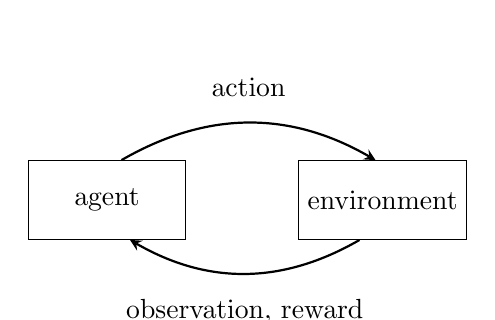
\begin{tikzpicture}[scale=1, transform shape, node distance=2.0cm]
		\node (agent) [rec] {agent};
		\node (environment) [rec, right of=agent, xshift=1.5cm] {environment};
		\draw [arrow, xshift=0.5cm]  (environment.240) to [bend left=30] node [midway, below, yshift=-0.2cm] (textnode1) {observation, reward}  (agent.300);
		\draw [arrow, xshift=0.5cm]  (agent.70) to [bend left=30] node [midway, above, yshift=0.2cm] (textnode2) {action} (environment.100);
\end{tikzpicture}
\end{center}
\caption{Conceptual schematic of reinforcement learning.}
\label{fig:rl-shematic}
\end{figure}
Reinforcement learning is a 2-step iterative process.
The \textbf{agent}, which represents the computer program, takes \textbf{actions}
in its \textbf{environment}. It then \textbf{observes} the resulting state
of the environment and is also given a \textbf{reward}
which is a function mapping every state of the environment to a number.

To introduce reinforcement learning more formally,
we first describe the simplest possible problem 
to which reinforcement learning is the best solution.

\subsection{Bandit problems}
Reinforcement learning  uses training information that evaluates 
the actions taken rather than instruct by giving correct actions.
Consider this learning problem.
The agent is faced with $k$ different gambling slot machines.
Each of them give random rewards under an unknown distribution.
At each turn, the agents has to select one of the machines and pull its lever.
%The agents is repeatedly faced with a choice of k different actions.
%After each choice the agent receive a numerical reward based on the action selected.
The goal is to maximize the expected total reward over some number of turns.
%This is original form of k-armed bandit problem.
%Depending on the action selected $k$-armed bandit problem formalizes the value function to get the expected or average reward.
If the agent knew the distribution of rewards of each of the slot machines, 
it would simply choose the one with the highest expected reward in number of turns 
it has been given.
%It is assumed the agent do not know the action value with certainty although the estimate of 
%the action value is known by the agent and we expected it to be close to actual value of the action.
At any time step the agent will be able to select at least one action whose estimated value is greatest.
When the agent selects on of this actions it is exploiting the current knowledge of the
values of the actions.
If the agents keep exploiting the goal of maximizing reward over period of time will be trivial.
If instead the agent selects one of the non greedy action this will enables it to improve the average expected reward over time.
 
When addressing the canonical problem of sequential decision making under uncertainty,
the exploitation-exploration trade-off is highlighted.More specifically,
as depicted in Fig.1, an agent interacts with an unknown environment in a sequential manner to obtain rewards.
The ultimate goal is to maximize the rewards.
For one thing, the agent takes advantage of existing knowledge of the environment.
For another, the agent investigates an unfamiliar environment.
%Reinforcement Learning, which includes Multi-Armed Bandit (MAB), Markov Decision Process (MDP), and Partially observable Markov Decision Process, is always used to formalize the exploit-exploration trade-off (POMDP).

%\begin{figure}[H]
%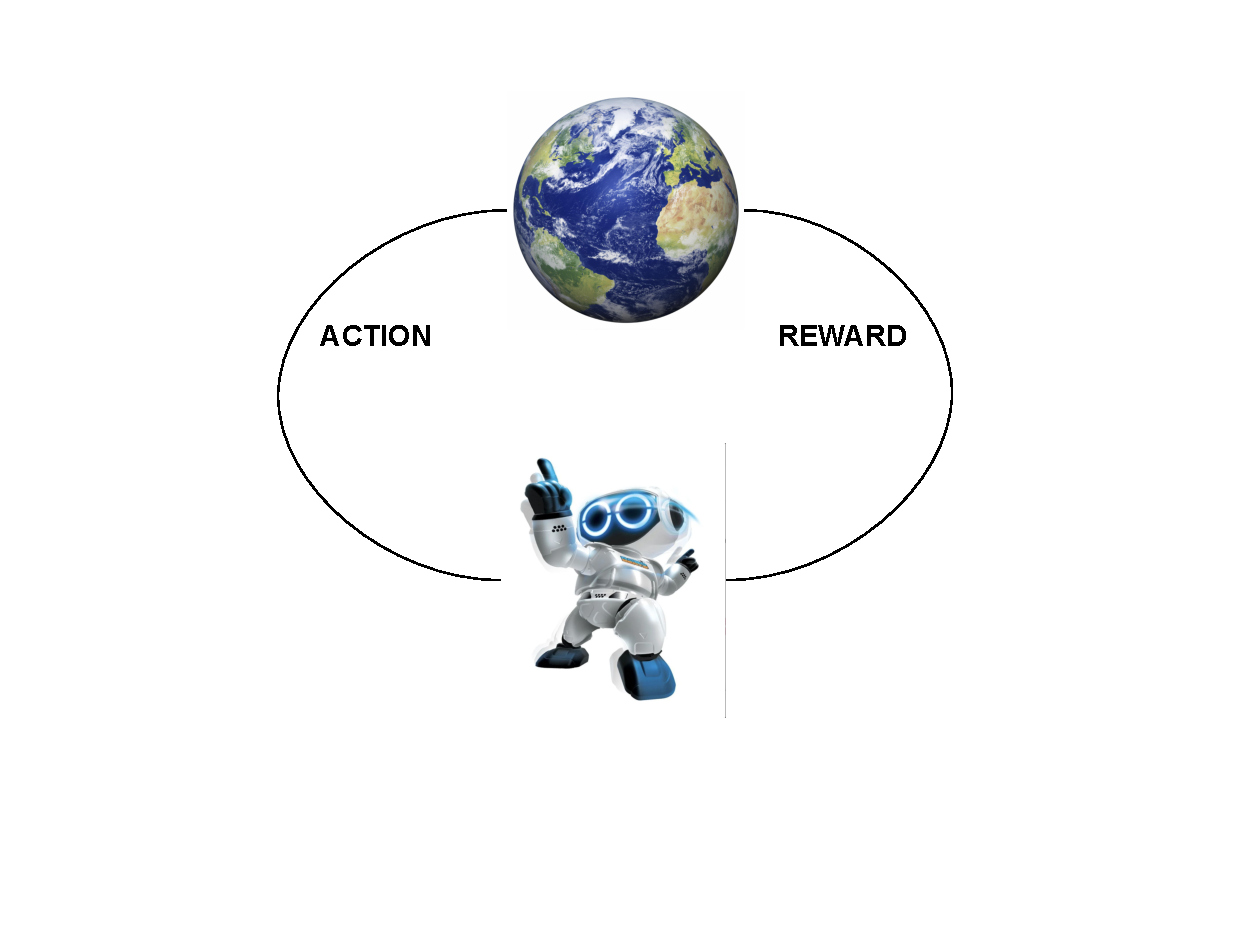
\includegraphics[width=12cm]{figure/RL_representation.pdf}
%\caption{An agent sequentially interaction with unknown environment and receive the rewards }
%\centering
%\end{figure}

%According to many studies of Reinforcement Learning,the unknown environment can described by multiple elements  including observations $\Omega$, states S, actions A, reward function R, state transition probability T, and conditional observation probabilities O.Bandit, MDP, and POMDP models the environment by considering different elements respectively.The formalisation of reward and policy in each model is different kinds of which leads to multiple techniques to learn.In the table 1  the relationship among bandit, MDP, RL, and decision theory are presented.In the next section we discuss the formalisation of MDPs for modern reinforcement learning.


\begin{table}[H]
\caption{Li Zhou ,relationship among bandit, MDP, RL, and decision theory}
\begin{tabular} {l|l|l}\hline\hline
$Learn model out come$  &  Mutlti armed bandits  &   RL \\ \hline
$Given model of stocastic out comes $ &  Decision Theory & MDP  \\ \hline\hline
$    $ &  Actions dont  
change state of the world & Actions change 
state of the world  \\ \hline\hline
\end{tabular}
\end{table}

%\textbf{TODO ADD EQUATION:
%   -FIT THE TABLE
%   -copy past the related work from the other notes
%   -rewrite some of the algorithms}
 
\subsection{Markov Decision Processes}
%\cite{gehring2017convolutional}
The environment of $ k  $-bandit problem is static --- 
the actions do not change the \textbf{state} of the environment.
To model environments in which states change, Markov chains are used.
They capture the stochastic nature of state transitions, while Markov property 
allows for easier mathematical analysis.
The schematic of a Markov chain is shown in \ref{fig:markov-chain}.

\begin{figure}[htpb]
\begin{center}
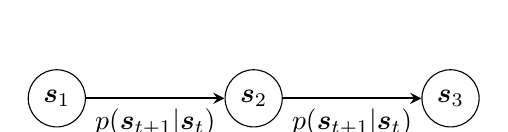
\begin{tikzpicture}[scale=1, transform shape, node distance=1.5cm]
		\node (s1) [mcs] {$\bm{s}_{1} $};
		\node (s2) [mcs, right of=s1, xshift=1cm] { $ \bm{s}_{2}  $};
		\draw [arrow] (s1) -- node [below, midway] {$ p(\bm{s}_{t+1}|\bm{s}_{t}) $} (s2);
		\node (s3) [mcs, right of=s2, xshift=1cm] { $ \bm{s}_{3}  $};
		\draw [arrow] (s2) -- node [below, midway] {$ p(\bm{s}_{t+1}|\bm{s}_{t}) $} (s3);
\end{tikzpicture}
\end{center}
\caption{Schematic of a Markov chain.}
\label{fig:markov-chain}
\end{figure}

Formally, a Markov chain $ \mathcal{M}  $is the defined by its state space
$ \mathcal{S}  $ with discrete or continous state $ \bm{s} \in \mathcal{S}  $
and the transition operator $ \mathcal{T}  $.
The notation $ \bm{s}_{ t }  $ denotes the state at time $ t  $ and it is a vector of real numbers.
The transition operator allow for a succinct description of environment dynamics.
For a transition probability $ p(s_{ t+1 }|s_{ t })  $,
let $ \mu_{ t,i } = p (\bm{s}_{t} = i)  $ and
$ \mathcal{T}_{ i,j } = p (\bm{s}_{t+1} = i|\bm{s}_{t} = j )  $.
Then $\overrightarrow{\mu}_t$ is a vector of probabilities and 
$\overrightarrow{\mu}_{t+1} = \mathcal{T} \overrightarrow{\mu}_t$.
Importantly, $ \mathcal{T}  $ is linear.

To model the agent's actions, we simply augment the Markov chain by adding
actions as priors to state transition probabilities and defining the reward function, 
thereby constructing a Markov decision process.
It's schematic can be seen in \ref{fig:mdp}.
\begin{figure}[htpb]
\begin{center}
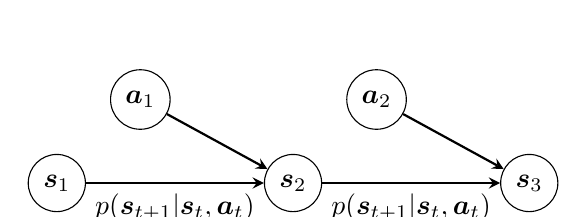
\begin{tikzpicture}[scale=1, transform shape, node distance=1.5cm]
		\node (s1) [mcs] {$\bm{s}_{1} $};
		\node (a1) [mcs, above right of=s1] { $ \bm{a}_{1}  $};
		\node (s2) [mcs, right of=s1, xshift=1.5cm] { $ \bm{s}_{2}  $};
		\draw [arrow] (a1) -- (s2);
		\draw [arrow] (s1) -- node [below, midway] {$ p(\bm{s}_{t+1}|\bm{s}_{t}, \bm{a}_{t}) $} (s2);
		\node (s3) [mcs, right of=s2, xshift=1.5cm] { $ \bm{s}_{3}  $};
		\node (a2) [mcs, above right of=s2] { $ \bm{a}_{2}  $};
		\draw [arrow] (s2) -- node [below, midway] {$ p(\bm{s}_{t+1}|\bm{s}_{t}, \bm{a}_{t}) $} (s3);
		\draw [arrow] (a2) -- (s3);
\end{tikzpicture}
\end{center}
\caption{Schematic of a Markov decision process.}
\label{fig:markov-chain}
\end{figure}

The Markov decision process is thus defined by the tuple
$ \mathcal{M} = \{\mathcal{S}, \mathcal{A}, \mathcal{T}, r\}  $.
$ \mathcal{A}  $ denotes the action space, where
$ \bm{a}_{} \in \mathcal{A}  $ is a continous or discrete action and
$ r  $ is the reward function $r : \mathcal{S} \times \mathcal{A} \to \mathbb{R}$.
It should also be noted that now the transition operator is a tensor.
Let $\mu_{t,j} = p(s_t = j), \xi_{t,k} = p(a_t = k), \mathcal{T}_{i,j,k} = p(s_{t+1} = i | s_t =j, a_t =k) $.
Then $\mu_{t+1,i} = \sum_{j,k}^{} \mathcal{T}_{i,j,k} \mu_{t,j} \xi_{t,k}$.
Hence $ \mathcal{T}  $ remains its linearity.

Finally, partial observability also needs to be accounted for.
To do so, a partially observable Markov decision process (POMDP) needs to be constructed.
This is done by augmenting the Markov decision process to also include
the observation space $ \mathcal{O}  $, where observations $ \bm{o}_{} \in \mathcal{O} $
denote the discrete or continous observations
and the emission probability $ \mathcal{E}  $ which describes the probability 
$ p(\bm{o}_{t} | \bm{s}_{t})  $ of getting the observation $ \bm{o}_{t}  $ when in state  $\bm{s}_{t}$.
The schematic can be seen in \ref{fig:pomdp}.

\begin{figure}[htpb]
\begin{center}
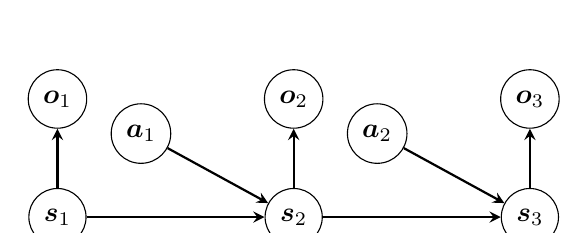
\begin{tikzpicture}[scale=1, transform shape, node distance=1.5cm]
		\node (s1) [mcs] {$\bm{s}_{1} $};
		\node (a1) [mcs, above right of=s1] { $ \bm{a}_{1}  $};
		\node (o1) [mcs, above of=s1] { $ \bm{o}_{1}  $};
		\draw [arrow] (s1) -- (o1);
		\node (s2) [mcs, right of=s1, xshift=1.5cm] { $ \bm{s}_{2}  $};
		\node (o2) [mcs, above of=s2] { $ \bm{o}_{2}  $};
		\draw [arrow] (s2) -- (o2);
		\draw [arrow] (a1) -- (s2);
		\draw [arrow] (s1) --  (s2);
		\node (s3) [mcs, right of=s2, xshift=1.5cm] { $ \bm{s}_{3}  $};
		\node (o3) [mcs, above of=s3] { $ \bm{o}_{3}  $};
		\draw [arrow] (s3) -- (o3);
		\node (a2) [mcs, above right of=s2] { $ \bm{a}_{2}  $};
		\draw [arrow] (s2) -- (s3);
		\draw [arrow] (a2) -- (s3);
\end{tikzpicture}
\end{center}
\caption{Schematic of a partially observable Markov decision process.}
\label{fig:pomdp}
\end{figure}
It is important to note that not all elements of POMDP are present in every problem: for example,
the reward may be a determinstic function of the state and so on.
In general through the text, to aid in simplifying notation, only the necessary elements will be explicity referenced
in sketches and written out in the equations (most often using just the Markov decision process).
%However, POMDP fully describes the setting in which reinforcement learning algorithms can be defined.


%Markov decision processes (MDPs) are used to model decision making in discrete, stochastic, sequential environments,
%and are thus a natural choice of model in which reinforcement learning can be defined.
%[9].
%Markov Chain, which works with S, a set of states, and P, the probability of transitioning from one to the next. It also uses the Markov Property, meaning each state depends only on the one immediately prior to it.

%MDPs is a framework that can solve most of reinforcement learning problems with discrete actions.The formal definition of Markov decision process can be summarised in  the tuple $\mathcal{M} = \{\mathcal{S}, \mathcal{A},\mathcal{P(S_0)}, \mathcal{T}, r\}$[8].
%The goal of the model is that an agent inhabits a  stochastic environment in a response to action choice made by the agent[9]. \\

%The environment consists of the the Transition function, $\mathcal{T} : \mathcal{S} \times \mathcal{A} \to \mathcal{(PS)}$.\\  and the reward function ($r(s_t, a_t)$), $r : \mathcal{S} \times \mathcal{A} \to \mathbb{R}$.In MDPs the transition probability and reward only depends on the current state and the action chosen by the agent  but not the past state and action.

%The agent acts in environment according to a policy $\mathcal{\pi} : \mathcal{S} \to \mathcal{(PS)}$.policy learned can be off policy where the behaviour policy is different from the policy used for action selection one common example is Q-learning or on-policy methods which attempts to evaluate or improve the policy that is used to make decision.\\
%The former state-action value function (Q function for short)can be computes recursively with dynamic programming: 


\subsection{Key concepts in reinforcement learning}
\subsubsection{Policy}
With the problem space being formally defined,
we may introduce definitions which will allow the construction
of reinforcement learning algorithm.
The reinforcement learning problem can be defined in finite or infinite time horizons.
Different environments usually naturally fall in either category.
For the agent to learn, it needs to be able to try out different actions from the same, 
or at least similar states.
This is usually achieved by having the agent return to a set of starting states.
The period between two such returns is called \textbf{an episode}.
The agent selects actions based on its \textbf{policy} $ \pi  $.
The policy is a function which maps states to actions.
The schematic showing it in the context of a Markov decision process
is given in \ref{fig:policy-in-mdp}.
\begin{figure}[htpb]
\begin{center}
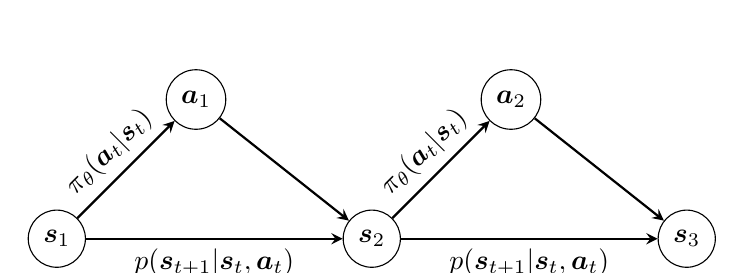
\begin{tikzpicture}[scale=1, transform shape, node distance=2.5cm]
		\node (s1) [mcs] {$\bm{s}_{1} $};
		\node (a1) [mcs, above right of=s1] { $ \bm{a}_{1}  $};
		\node (s2) [mcs, right of=s1, xshift=1.5cm] { $ \bm{s}_{2}  $};
		\draw [arrow] (a1) -- (s2);
		\draw [arrow] (s1) -- node [below, midway] {$ p(\bm{s}_{t+1}|\bm{s}_{t}, \bm{a}_{t}) $} (s2);
		\node (s3) [mcs, right of=s2, xshift=1.5cm] { $ \bm{s}_{3}  $};
		\node (a2) [mcs, above right of=s2] { $ \bm{a}_{2}  $};
		\draw [arrow] (s2) -- node [below, midway] {$ p(\bm{s}_{t+1}|\bm{s}_{t}, \bm{a}_{t}) $} (s3);
		\draw [arrow] (a2) -- (s3);
		\draw [arrow] (s1) -- node [above, midway, sloped] {$\pi_{ \theta } (\bm{a}_{t}| \bm{s}_{t} )  $} (a1);
		\draw [arrow] (s2) -- node [above, midway, sloped] {$\pi_{ \theta } (\bm{a}_{t}| \bm{s}_{t} )  $} (a2);
\end{tikzpicture}
\end{center}
\end{figure}

The policy is a stochastic function. The intensity of stochasticity determines the trade-off
between exploration and exploitation.
To emphasize that the policy depends on some parameters $ \theta  $,
we usually write $ \pi_{ \theta } $.

\subsubsection{Goal of reinforcement learning}
For simpler notation, the finite horizon form
is assumed for the following definitions.
Since the environment is modelled as a Markov decision process,
we can write the probabily of observing a trajectory of states
and actions as:

\begin{equation}
\underbrace{p_\theta(\bm{s}_1, \bm{a}_1, \dots, \bm{s}_T, \bm{a}_T)}_{p_\theta(\tau)} = p(\bm{s}_1) \prod^{T}_{t=1} 
\underbrace{\pi_{\theta} (\bm{a}_t | \bm{s}_t) p (\bm{s}_{t+1} | \bm{s}_t, \bm{a}_t)}_{\text{Markov chain on} (\bm{s}, \bm{a})}
\end{equation}
A bit more explicitely, we can a transition probaility as:
\begin{equation}
p((\bm{s}_{t+1}, \bm{a}_{t+1}) | (\bm{s}_t, \bm{a}_t)) = 
p((\bm{s}_{t+1}| (\bm{s}_t, \bm{a}_t)) \pi_\theta (\bm{a}_{t+1} | \bm{s}_{t+1})
\end{equation}

With this, we may now formally define the goal of reinforcement learning.
It is to find policy parameters $ \theta^{ \star }  $ such that:
\begin{align}
		\theta^\star &= \argmax_{\theta} E_{\tau \sim p_\theta(\tau)} \left[ \sum_{t}^{} r(\bm{s}_t, \bm{a}_t) \right] \\
	 &= \argmax_{\theta} \sum_{t}^{T} E_{(\bm{s}_t, \bm{a}_t) \sim p_\theta(\bm{s}_t, \bm{a}_t)} \left[  r(\bm{s}_t, \bm{a}_t) \right]
\end{align}

To ensure that the expected sum of rewards, also know as the \textbf{return},
is finite in the infinite horizon case, a
\textbf{discount factor} $ 0 < \gamma < 1  $ is introduced in the sum.
The discount factor also play a role in modelling 
because often times it makes sense to value immediate rewards
more.
It is important to note that we are maximizing the \textit{expected} sum of
rewards. This it a the goal a smooth and differentiable function of the parameters,
which means we can employ gradient descent to find the optimal parameters.
This leads us to the first class of reinforcement learning algorithms:
policy gradient algorithms.
They will be introduced with the other classes of algorithm in the next subsection,
while here additional concepts required by other classes of algorithms will be introduced here.

\subsubsection{Value functions}
Value functions are functions which map states or state-action pairs
to the expected returns obtained under a fixed policy.
They are a concept from dynamic programming. In fact,
reinforcement learning can be interpreted as an extension of dynamic programming,
as shall be done in the following subsection.
Having that said, value function can be interpreted in other ways as well.
The \textbf{Q-function} maps state-action pairs to the estimated sum of returns
under policy $ \pi_{ \theta } $:
\begin{equation}
		\label{eq:q-function}
		Q^\pi (\bm{s}_t, \bm{a}_t) = \sum_{t'=t}^{T} E_{\pi_\theta}
		\left[ r(\bm{s}_{t'}, \bm{a}_{t'} )| \bm{s}_t, \bm{a}_t \right] 
\end{equation}
thus denoting the total reward from taking $\bm{a}_t$ in $\bm{s}_t$.
\textbf{Value functions} map states to to the estimated sum of returns
under policy $ \pi_{ \theta } $:
\begin{equation}
		\label{eq:value-function}
		V^\pi (\bm{s}_t) = \sum_{t'=t}^{T} E_{\pi_\theta}
		\left[ r(\bm{s}_{t'}, \bm{a}_{t'} | \bm{s}_t) \right] 
\end{equation}

The connection between the two is the following:
\begin{equation}
		V^\pi (\bm{s}_t) = E_{\bm{a}_t \sim \pi(\bm{s}_t, \bm{a}_t)}
		\left[ Q^\pi(\bm{s}_t, \bm{a}_t) \right] 
\end{equation}
And we can also write the RL objective as:
\begin{equation}
		E_{\bm{s}_1 \sim p(\bm{s}_1)}
		\left[ V^\pi (\bm{s}_1) \right] 
\end{equation}


\section{Classes of reinforcement learning algorithms}
\subsection{Policy gradients}
Policy gradients are derived by directly solving for
the reinforcement learning objective with gradient descent
with respect to the policy parameters.
To do so, the reinforcement learning objective needs to be evaluated.
We begin by introducing a notational shorthand:

\begin{equation}
		\theta^\star = \argmax_\theta \underbrace{E_{\tau \sim p_\theta (\tau)} \left [ \sum_t r(\bm{s}_t, \bm{a}_t) \right ]}_{J(\theta)}
\end{equation}

We estimate $J(\theta)$ by making rollouts from the policy (below $i$ is the sample index and $i,t$ is the $t^{th}$ timestep
in the $i^{th}$ sample):
\begin{equation}
		J(\theta) = E_{\tau \sim p_\theta(\tau)} \left [ \sum_t r(\bm{s}_t, \bm{a}_t) \right ] \approx 
		\frac{1}{N} \sum_i \sum_t r(\bm{s}_{i,t}, \bm{a}_{i,t})
\end{equation}
Simplifying the notation further, we get:
\begin{equation}
		J(\theta) = E_{\tau \sim p_\theta(\tau)} \underbrace{[r(\tau)]}_{\sum^{T}_{t=1} r(\bm{s}_t, \bm{a}_t)} = 
		\int_{{}}^{} {p_\theta(\tau)r(\tau)} \: d{\tau} {}
\end{equation}
The goal now is to compute the derivative of the estimated reinforcement learning
objective:
\begin{equation}
		\label{eq:derivative-of-estimated-rl-obj}
		\nabla_\theta J(\theta) = \int_{{}}^{{}} {\nabla_\theta p_\theta (\tau) r(\tau)} \: d{\tau} {}
\end{equation}

Since the goal of this text is just to introduce the necessary concepts
and algorithms, the derivation(s) will be ommited.
We encourage the interested reader to consult the literature \cite{suttonrlbook}
and CITE LEVINE'S BERKLEY LECTURES to find them.
Here we will just note that it is crucial that the final expression
can be estimated by sampling the agent's experience 
as the other quantities are not available.
The resulting expression for the policy gradient \label{eq:derivative-of-estimated-rl-obj} is:

\begin{equation}
		\label{eq:policy-gradient}
		\nabla_\theta J(\theta) = E_{\tau \sim p_\theta(\tau)} 
		\left [ \left ( \sum_{t=1}^{T} \nabla_\theta \log \pi_\theta (\bm{a}_t | \bm{s}_t ) \right )
		\left ( \sum_{t=1}^{T} r(\bm{s}_t, \bm{a}_t) \right ) \right ]
\end{equation}
To evaluate the policy gradient we can sample:
\begin{equation}
		\label{eq:estimated-policy-gradient}
		\nabla_\theta J(\theta) \approx \frac{1}{N}  \sum_{i=1}^{N} 
		\left ( \sum_{t=1}^{T} \nabla_\theta \log \pi_\theta (\bm{a}_{i,t} | \bm{s}_{i,t} ) \right )
		\left ( \sum_{t=1}^{T} r(\bm{s}_{i,t}, \bm{a}_{i,t}) \right )
\end{equation}
With the gradient we can do a step of gradient ascent and use it to form
the REINFORCE algorithm, also known as ``vanilla policy gradient'':

\fbox{
		\parbox{\textwidth}{
				\underline{REINFORCE algorithm:}
\begin{enumerate}
		\item sample $\{\tau^i\}$ from $\pi_\theta(\bm{a}_t | \bm{s}_t)$ by running the policy
		\item $\nabla_\theta J(\theta) \approx   \sum_{i}^{} 
		\left ( \sum_{t}^{T} \nabla_\theta \log \pi_\theta (\bm{a}_{i,t} | \bm{s}_{i,t} ) \right )
		\left ( \sum_{t}^{} r(\bm{s}_{i,t}, \bm{a}_{i,t}) \right )$
\item $\theta \leftarrow \theta + \alpha \nabla_\theta J(\theta) $
\end{enumerate}
}}

This algorithm does not work well in practice.
The main reason for that is that the variance of returns
is very high. 
However, there are a number of modification
which dramatically improve its performance.
Since the goal of this text is not to outline every reinforcement learning algorithm,
we will introduce only the modifications which outline
general trade-offs and principles in reinforcement learning algorithm design.

\subsubsection{Baselines}
The policy gradient in the REINFORCE algorithm lacks some important properties.
One of them is that it should, ideally, make bad actions less likely
and good actions more likely. 
However, if all rewards are positive, then all action's probabilites will be increased,
only by different amounts.
This can be changed if a \textbf{baseline} $ b  $is added to actions:
\begin{align}
		\nabla_\theta J(\theta) &\approx 
		\frac{1}{N} \sum_{i=1}^{N}
		\nabla_\theta \log p_\theta (\tau) [ r(\tau) - b] \\
		b &= \frac{1}{N} \sum_{i=1}^{N} r(\tau)
\end{align}
This addition doesn't change the gradient in expectation, i.e. it does not
introduce bias,
but it does change its variance.
While an optimal bias can be calculated, it is rarely used in practise due
to its computational cost.
Using baselines is one of the key ideas in actor-critic algorithms
so they will be discussed further there.

\subsubsection{Off-policy gradients}
An important property of the REINFORCE algorithm is that it
is an \textbf{on-policy} algorithm.
This means that new samples need to be collected for every gradient step.
The reason behind this is the fact that the expectation of the gradient 
of the return needs to be calculated with respect to the current parameters
of the policy.
In other words, because the policy changes with each gradient step,
old samples are effectively collected under a different policy.
This means that they can not be used to calculate the expected gradient 
of the return with respect to the current policy --- it would not
produce those trajectories.
In mathematical notation:
\begin{equation}
		\nabla_\theta J(\theta) = \underbrace{E_{\tau \sim p_\theta(\tau)}}_{\text{this is the trouble!}} [\nabla_\theta p_\theta(\tau)r(\tau)]
\end{equation}
If the policy is a neural network, which requires small gradient steps,
the cost of generating a big number of samples for every update
could make the algorithm entirely infeasible.
This of course depends on the cost of generating samples,
which is entirely problem dependent ---
policy gradient algorithms are often the best solution when 
the cost of generating samples is low.

However, on-policy algorithms can be turned into off-policy 
algorithms through \textbf{importance sampling},
which is the name given to the following mathematical identity:
\begin{align}
		E_{x \sim p(x)} [f(x)]  
		&= \int_{{}}^{{}} {p(x)f(x)} \: d{x} \\
		&= \int_{{}}^{{}} {\frac{q(x)}{q(x)}  p(x)f(x)} \: d{x} \\
		&= \int_{{}}^{{}} { q(x) \frac{p(x)}{q(x)}  f(x)} \: d{x} \\
		&= E_{x \sim p(x)} \left [ \frac{p(x)}{q(x)} f(x) \right ]
\end{align}
which is exact in expectation.
To use importance sampling to create an off-policy policy gradient algorithm,
certain approximations need to be made. Again, the details of the derivation
are ommited and what follows is just the final result.
\begin{equation}
		\nabla_{\theta'} J(\theta') \approx
		\frac{1}{N} \sum_{i=1}^{N} \sum_{t=1}^{T}
		\frac{\pi_{\theta'}( \bm{a}_{i,t} | \bm{s}_{i,t})}{\pi_{\theta}( \bm{a}_{i,t} | \bm{s}_{i,t})} 
		\nabla_{\theta'} \log \pi_{\theta'} (\bm{s}_{i,t}, \bm{a}_{i,t}) 
		\hat{Q}_{i,t} 
\end{equation}
To get this equation, the factor 
$ \frac{\pi_{\theta'}(\bm{s}_{i,t})}{\pi_{\theta}(\bm{s}_{i,t})}  $
had to be simple ignored in the expression because it is impossible 
to calculate the state marginal probabilities.
This means that the expression works only if $ \pi_{ \theta' }  $
is not too different from $ \pi_{ \theta }  $.

\paragraph{Advanced policy gradient}
The basic algorithm we have outline is essentially just a basic
gradient descent method. 
From convex optimization, we know that it can be made much better if second order derivatives
or their approximations are used.
For example, conjugate gradient descent can be used.
Further, there are various ways in which this optimization problem can be better conditioned.
Such improvements led algorithms such as PPO and TRPO,
which will not be discussed here.

\subsection{Actor-critic algorithms}
Actor-critic methods can be seen as making a different trade-off between 
variance and bias in policy gradient estimation.
We begin with the following observation:
\footnote{In this equation, the summation of rewards is done from time $t   $
		to $ T  $ because actions and states prior to that time do
		not affect the return from that time onward.
This leveraging of causality reduces the variance of the estimate.}
\begin{equation}
		\nabla_\theta J(\theta) \approx 
		\frac{1}{N} \sum_{i=1}^{N} \sum_{t=1}^{T} \nabla_\theta \log \pi_\theta (\bm{a}_{i,t}| \bm{s}_{i,t})
		\underbrace{\left ( \sum_{t'=t}^{T} r (\bm{s}_{i,t}, \bm{a}_{i,t}) \right )}_{\hat{Q}_{i,t}
		\text{: ``reward to go''}}
\end{equation}
Simply put, in the policy gradient method a single-run Monte-Carlo (MC) is used
to estimate the return.
This causes high variance, while incurring no bias.
Another option is to try to estimate the full expectation
$ \hat{Q}_{i,t} \approx  \sum_{t'=t}^{T} E_{\pi_\theta} \left[ r(\bm{s}_{t'}, \bm{a}_{t'}) |\bm{s}_{t}, \bm{a}_{t}  \right]     $.
Since the estimate won't be perfect, it will introduce bias.
Of course, using multiple runs from the same state-action pair would 
reduce variance, but this is sometimes impossible to procure
and is certainly more costly.
However, if our estimator of ``reward to go'' can generalize between states,
we will be able to get good estimates regardless.

Like the policy, the return estimator will have to be learned.
In this approach, the policy is also called the \textbf{actor} 
and the return estimator is called the \textbf{critic}.
We proceed by discussing how the critic can be constructed.
If we had the correct Q-function (i.e. not the estimate, but the actual values),
we could improve the policy gradient estimate by using it
both to estimate the return and as a baseline:
\begin{align}
		\nabla_\theta J(\theta) &\approx \frac{1}{N} \sum_{i=1}^{N} \sum_{t=1}^{T} \nabla_\theta \log \pi_\theta (\bm{a}_{i,t}| \bm{s}_{i,t})
( Q(\bm{s}_{i,t}, \bm{a}_{i,t}) - b) \\
		b_t &= \frac{1}{N} \sum_{i}^{} Q(\bm{s}_{i,t}, \bm{a}_{i,t})
\end{align}
However, having a baseline that depends on actions leads to bias.
Thus we employ a baseline dependent on the state:
\begin{equation}
		V(\bm{s}_t) = E_{\bm{a}_t \sim \pi_\theta (\bm{s}_{t}, \bm{a}_{t})} [Q(\bm{s}_{t}, \bm{a}_{t})]
\end{equation}
Since the value function \ref{eq:value-function} tells us the expected return of the average action,
we can calculate how much better a certain action is by substracting
its Q-value \ref{eq:q-function} for the value function.
The result is called the \textbf{advantage function}:
\begin{equation}
A^\pi (\bm{s}_{t}, \bm{a}_{t}) = Q^\pi (\bm{s}_{t}, \bm{a}_{t}) - V^\pi (\bm{s}_t)
\end{equation}
Thus we can fit either the Q-function, the value function or the advantage function.
Of these, it is best to learn the value function because there are less 
states than state-action pairs.
We then calculate the advantage function in the following way:
\begin{align}
		A^\pi (\bm{s}_{t}, \bm{a}_{t})  &\approx r(\bm{s}_{t}, \bm{a}_{t}) + V^\pi (\bm{s}_{t+1})  - V^\pi(\bm{s}_t)
\end{align}

The value function can be estimated through samples
\begin{align}
		V^\pi (\bm{s}_t) &\approx \sum_{t'=t}^{T} r(\bm{s}_{t'}, \bm{a}_{t'})
\end{align}
After collecting many such samples
\begin{equation}
		\left\{ \left( \bm{s}_{i,t}, \underbrace{\sum_{t'=t}^{T} r(\bm{s}_{i,t}, \bm{a}_{i,t})}_{y_{i,t}} \right)  \right\} 
\end{equation}
we can fit the value function through supervised regresion with the loss being:
\begin{equation}
		\mathcal{L}(\phi) = \frac{1}{2} \sum_{i}^{} ||\hat{V}^\pi_\phi (\bm{s}_i) - y_i||^2
\end{equation}
However, this process can be sped up with bootstraped estimates:
\begin{equation}
		y_{i,t} = \sum_{t'=t}^{T} E_{\pi_\theta} \left[ r(\bm{s}_{t'}, \bm{a}_{t'})|\bm{s}_{i,t}\right] + V^\pi(\bm{s}_{i,t+1})  
		\approx r(\bm{s}_{i,t}, \bm{a}_{i,t}) + \hat{V}^\pi_\phi(\bm{s}_{i,t+1}) 
\end{equation}
This will further reduce variance, but again increase bias.

Fortunatelly, we can tune the trade-off between bias and variance.
In the Monte Carlo estimate, the entire trajectory was used
to estimate the return. In the bootstrap estimate,
only a single step in the future was used along with the estimate.
Instead, a \textbf{n-step} return estimator can used:
\begin{equation}
		\hat{A}^\pi_n (\bm{s}_{t}, \bm{a}_{t}) =
		\sum_{t'=t}^{t+n} \gamma^{t'-t} r(\bm{s}_{t'}, \bm{a}_{t'})
		- \hat{V}^\pi_\theta(\bm{s}_t) + \gamma^n \hat{V}^\pi_\theta(\bm{s}_{t+n})
\end{equation}
In most cases
the ideal trade-off for $ n  $ lies somewhere between 1 and $\infty$ (the MC estimate).
Finally, an average of all n-step return estimators can be used.
This is called the generalized advantage estimator (GAE):
\begin{equation}
\hat{A}^\pi_{GAE} (\bm{s}_{t}, \bm{a}_{t}) =
\sum_{n=1}^{\infty} (\gamma \lambda)^{t'-t}r(\bm{s}_{t'}, \bm{a}_{t'}) + \gamma \hat{V}^\pi_\theta(\bm{s}_{t'+1})  - \hat{V}^\pi_\theta(\bm{s}_{t'})
\end{equation}
where the factor $ \lambda  $ controls the weight of future values.

Combining this into an iterative algorithm, and fixing the issues
of naiive implementations results in the following algorithm:

\fbox{
\parbox{\textwidth}{
\underline{Actor-critic algorithm template}
\begin{enumerate}
		\item take action $\bm{a} \sim \pi_\theta(\bm{a}|\bm{s})$, get $(\bm{s}, \bm{a},\bm{s'},r)$, store in $\mathcal{R}$ (replay buffer)
		\item sample a batch $\left\{  (\bm{s}_i, \bm{a}_i,\bm{s'}_i,r_i) \right\} $ from buffer $\mathcal{R}$
		\item update $\hat{Q}^\pi_\theta$ using target $y_i = r_i + \gamma \hat{Q}^\pi_\theta(\bm{s}_i', \bm{a}_i') \forall \bm{s}_i, \bm{a}_i$
		\item $\nabla_\theta J(\theta) \approx  \frac{1}{N} \sum_{i}^{}  \nabla_{\theta} \log \pi_\theta(\bm{a}^\pi_i|\bm{s}_i)\hat{Q}^\pi(\bm{s}_{i}, \bm{a}^\pi_{i})$,
				where $\bm{a}_i^\pi \sim \pi_\theta(\bm{a} | \bm{s}_i)$
		\item $\theta \leftarrow \theta  + \alpha \nabla_\theta J(\theta)$
\end{enumerate}
}}

%\begin{equation}
%   	Q^\pi (s,a) = E_s'[r + \gamma E_a'~\pi(s') [Q^\pi(s',a')]|s,a,\pi]
%\end{equation}
 
%optimal q value under deterministic policy
%\begin{equation} 
%a = argmax_a'\epsilon A Q^*(s,a')
%\end{equation} 
%
%\begin{equation}
%	  Q^* (s,a) = \max_\pi  Q^\pi(s,a)
%\end{equation}
%
%if the optimal function satisfies the bellman equation:
%\begin{equation}
%    Q^* (s,a) = E_s' [r + \gamma max(\bm{a'}) Q^* (s',a')| s,a,\pi]
%\end{equation}
%
%The advantage function  describes “how good” the action a is, compared to the expected return when following direct policy pi.
%
%\begin{equation}
%    A^\pi (s,a) = Q^\pi(s,a)- V^\pi(s)
%\end{equation}
%
%The value function V measures the how good it is to be in a particular state s. The Q function, however, measures the the value of choosing a particular action when in this state[6].\\

\subsection{Value function methods}
Value function methods use only the critic from actor-critic algorithms.
Suppose that the advantage function $ A^{ \pi } (\bm{s}_{t}, \bm{a}_{t} )  $ is known.
It tells us how much better the action $ \bm{a}_{t}  $ is than the average action
according to the policy $ \pi  $.
Thus, if we knew the advantage function, we could construct a deterministic 
\textbf{greedy policy}:
\begin{equation}
		\pi_{ \text{greedy} }(\bm{s}_{t}| \bm{a}_{t}) = \left\{ 
\begin{matrix}
		1 & \text{ if } \bm{a}_t = \argmax_{\bm{a}_t} A^\pi (\bm{s}_{t}, \bm{a}_{t}) 		 \\
		0 & \text{ otherwise}
\end{matrix}
		\right.
\end{equation}
which would yield the highest expected return.
In other words, if we knew the advantage function, the policy would be
reduced to the argmax operation.

\subsubsection{Dynamic programming}
Dynamic programming refers to a collection of algorithms that can be used
to compute optimal policies given a perfect model of the environment as
an MDP.
They are of limited utility in reinforcement learing due to the perfect model requirement 
and their great computational expense, but are important theoretically ---
they provide an essential foundation for understanding the other methods.
Usually a finite MDP is assumed. DP can be applied to continous problems as well,
but exact solution exist only in special cases.

TODO: 
\begin{enumerate}
		\item Introduce value iteration in a tabular setting
		\item introduce fitted value iteration
		\item show that q-learning is off-policy
		\item show that q-learning does not converge when using non-linear function
				approximation (introduce the bellman operator as well)
\end{enumerate}

\section{Deep Reinforcement Learning and DQN}

(paraphrase)After deep learning  has shown remarkable results in learning from raw pixel data in computer vision it's application has been adopted to solve many classical learning problems.The goal of Deep Reinforcement Learning is to connect reinforcement learning algorithm to deep neural network which operates directly on RGB images and efficiently process training data by using stochastic gradient updates[2].\\

The use of label data and the assumption the distribution of data to be identical and independent through out training process in deep learning makes it complex to use it directly into reinforcement learning algorithms which must be able to learn from sparse ,noisy and delayed reward and highly correlated data.To address this issues and successfully apply deep learning to reinforcement learning [2] used experience replay mechanism[15] which randomly samples previous transitions, and thereby smooths the training distribution over many past behaviors.Convolutional neural network was used to  learn successful control policies from raw video data in complex reinforcement learning environment.The network is trained with a variant of Q-learning algorithm,with stochastic gradient descent to update the weights.

This architecture was based on Tesauro’s TD-Gammon architecture [17]
which updates the parameters of the network that estimates the value function 
directly from on-policy samples of experience. 
Similar to this approach the online network  in DQN utilize a 
technique known as experience replay [18] where the 
agent’s experiences at each time-step, 
$\mathcal e_t = (s_t,a_t,r_t,s_t+1)$ is stored in a data set 
$\mathcal D = e1 , ..., e_N $ pooled over many 
episodes into a replay memory.
By drawing random samples from this pool of stored experiences  the Q-learning is updated.
After performing experience replay, the agent selects and executes an 
action according to an $\epsilon$-greedy policy.
The use of experience replay and target networks enables 
relatively stable learning of Q values, 
and led to super human performance on several Atari games.

The advantage of using Deep Q-learning over Q-learning  
includes allowing  to have greater sample efficiency,
reduced variance by randomising the sample bias and avoiding being 
stuck in local minimum.Drawback  
DQNs are it only handle discrete,low-dimensional action space.


\subsection{Extension of DQN }

Several Studies were performed to increase the performance of DQNs(Paraphrase).

\subsubsection{Double Deep Q-networks: DDQN}

DQN suffer from overestimation bias due to due to the maximization step in optimisation function in Q-learning.Q-learning can overestimate actions that have been tried often and the estimations can be higher than any realistic optimistic estimate .Double Q-learning [19], addresses this overestimation by decoupling, in the maximization performed for the bootstrap target, the selection of the action from its evaluation.Double Q-learning stores two Q-functions,The average of the two Q values for each action and then performed $\mathcal{\epsilon}$-greedy exploration with the resulting average Q values.It was successfully combined with DQN to reduce  overestimations.\textbf{ TODOS: DDQN  target equation}

\subsubsection{Prioritized replay}

The main use of replay buffer is to sample transitions with maximum probability.Both DQN and DDQN samples experiences uniformly.Prioritized replay [20] samples transitions using the maximum priority ,providing a bias towards recent transitions and stochastic transitions  even when there is little left to learn about them.

\subsubsection{Dueling Network}

Dueling Network was designed for  value based learning,this architecture separates the representation of sate-value and state-dependent action advantages without supervision[6].its consists of two streams that represents the value and advantage functions,while sharing a common convolutional feature learning module.This network has a single Q-learning network with two streams that replace DQN architecture[3]. 

\begin{equation}
    Q(s,a; \theta,\alpha,\beta) = V(s,\theta,\beta) + A(s,a; \theta,\alpha)
\end{equation}

\textbf{if needed TODO ADD EQUATION:factorization of action values}

\subsubsection{Multi-step learning}

Previously stated extension of DQN have indicated that the use deep learning has enhanced the learning capability of Q-learning.The performance of  Q-learning is still limited by greedy action selection after accumulating a single reward.An alternative approach was multi-step targets:
 
 \begin{equation}
		y_{j,t} = \sum_{t'=t}^{t+N-1} \gamma^{t-t'}    r_{j,t'} + \gamma^N  \max_{\bm{a}_{j,t+N}}Q_{\phi'}(\bm{s}_{j,t+N}, \bm{a}_{j,t+N}) 
\end{equation}

A multi-step variant of DQN is then defined by minimizing
the alternative loss[16],

\begin{equation}
	    R_t^{(n)} +  \gamma_t^{(n)}  \max_{a'} q_\theta^{-}(S_{t+n},a') - q_{\theta}(S_t,A_t)
\end{equation}
  

\subsubsection{Noisy Nets}

The one limitation of $\mathcal{\epsilon}$-greedy policy  is many actions must be executed to collect the first reward.Noisy Nets proposed a noisy linear layer that combines  a deterministic and noisy stream.Depending on the learning rate the network ignores to learn the noisy stream.

\subsubsection{Integrated Agent:Rainbow}


In the Rainbow architecture [16]  tries combine the above six 
method stated above all together.Distributional loss (3) 
was replaced with a multi-step variant.
The target distribution was constructed  by contracting the value distribution 
in St+n according to the cumulative discount, 
and shifting it by the truncated n-step discounted return. 
multi-step distributional loss with double Q-learning by using the greedy action in St+n 
selected according to the online network as the bootstrap action $a \cdot t+n,$ and evaluating such action using the target network.

\textbf{TODO ADD EQUATION:target distribution}

\section{Problems with RL}
ex. drl that matters paper

\section{general computer vision stuff}

\section{general latent space learning}
summarize this
\cite{staterepresentationlearningoverview}


\section{Related Work}
todo, not sorted:
related to us
\begin{enumerate}
		\item algs we use: \cite{erainbow}, \cite{sac}
		\item (us) yarats improving sample efficiency \cite{sac+ae}, \cite{laser}
		\item (us as inspiration) \cite{icm}
		\item (not us but same high-level idea): data-augmentation like \cite{drqv2}, 
				contrastive loss like \cite{curl}, \cite{rad},
				\cite{flow}, \cite{imageaugmentationisallyouneed}
		\item (not us, but things that can be done with image loss): \cite{lossisitsownreward}
		\item (discuss some state of the art ); \cite{agent57}
		\item (us, historic) deep Auto-Encoder Neural Networks in Reinforcement Learning 
				\cite{firstaeinrl}
\end{enumerate}
sort these in the bellow two sections

\subsection{Current state-of-the-art}


\subsection{Related to our work}











\section{General latent space learning}
TODO: throw in citations (ex. pilco, embed2control etc)

As discussed in the introduction, learning control from images is 
very desirable. Images, and observations in general, only implicitely 
provide information about the underlying state. 
Finding a good policy from observations, especially images,
is much more difficult than finding a policy with direct state access
because the state first needs to be infered from those observations.
Reinforcement learning algorithms can by themselves implicitely extract
the relevant information from observations, but this at best results
in much less sample-efficient training and at worst results
in complete failure.
Often a problem which a reinforcement learning algorithm can solve
with direct state access, can not achieve any progress when
provided only image observations.

It is clear from the previous section that
amazing results were achieved in the field of computer vision.
However, to leverage these results for the purposes of reinforcement
learning, the methods in question need to be applied for state estimation.
This is a drastically different problem than for example image classification.
The key difference is that now dynamics need to be inferred.
While neural network arhictectures like the convolutional neural network
are able to achieve great successes in timeless problems, 
neural architectures like LSTMs aimed at learning from sequential data
comparatively perform much worse.
Results in problems such as video prediction or action classification leave much to be desired.

Having that said, the learning signal generated from for example
image reconstruction loss is substantially stronger than the reward signal,
especially in settings with sparse rewards where it is 
not present most of the time.
Thus it stands to reason that somehow leveraging the learning
signal from some computer vision method should aid the reinforcement learning 
process. 
One way to do this is to explicitely use such methods to learn 
a function which maps from observations to states
and then use reinforcement learning methods these learned state
represetantions.
This approach is explored in this section, mainly with the help
of the 
\cite{staterepresentationlearningoverview}
overview paper.
Here we discuss state represetantion learning for control in general
as this will allow for a broader contextualization of our own work.
Importantly, this does not concern learning a model 
which can be used to achieve control through planning,
altough there are of course similarities between these approaches.

In general, represetantion learning algorithm are designed to learn
abstract features that characterize data.
In the simplest forms they include methods such as k nearest neighbors.
In state represetantion learning (SRL) the learned features
are of low dimension, evolve through time and are depended
on actions of an agent.
The last point is particularly important because in reinforcement learning,
features that do not influence the agent and that can not be influenced
by the agent are not relevant for the problem of optimally controlling the agent.
Also, simply reducing the dimensionality of the input to a reinforcement learning
agent results in a computationally easier learning problem,
which can make a difference between the solution being feasible or infeasible.
Ideally, state  represetantion learning should be done in an without explicit supervision
as it can then be done in tandem with the likewise unsupervised reinforcement learning.

While we assume that state-transitions have the Markov property,
partial observability denies the possibility of having a one-to-one
correspondence between each observation and state ---
an object whose position is required may be occluded by another.
Thus prior observations have affect the mapping to the current state.
Images in particular also do not encode kinematic or dynamic information:
to get that crucial information a sequence of images is required.
Hence we define the SRL task as learning
a represetantion $ \tilde{\bm{s}}_{t} \in \tilde{\cal{S}}  $ of dimension $ K  $
with characteristics similar to those of true states $ \bm{s}_{t} \in \mathcal{S} $.
In particular, the represetantion is a mapping of the history of 
observation to the current state: $ \tilde{\bm{s}}_{t} = \phi(\bm{o}_{1:t}  $.
Actions $ \bm{a}_{1:t}  $ and rewards $ r_{ 1:t }  $ can also be added
to the parameters of $ \phi  $.
This can help in extracting only the information relevant for the agent and its task.
Often the represetantion is learned by using the reconstruction loss;
$ \hat{\bm{o}_{t}}  $ denotes the reconstruction of $ \bm{o}_{t}  $.

In the context of reinforcement learning, state representations should
ideally have the following properties:
\begin{itemize}
		\item have the Markov property 
		\item be able to represent the current state well enough for policy improvement
		\item be able to generalize to unseen states with similar features
		\item be low dimensional
\end{itemize}

With this we can introduce 4 different stategies for learning latent space models:
the auto-encoder, the forward model, the inverse model and the model
with prior.
In the figures below, the white nodes are inputs and the gray nodes are outputs.
The dashed rectangles are fitted around variables with which the loss is calculated.

\subsection{Auto-encoder}
The idea behind the auto-encoder is to just learn a lower-dimensional embedding
of the observation space. This should make the learning problem easier due to the
dimensionality reduction.
The auto-encoder may be trained to denoise the observations by passing an observation
with artificially added noise to the encoder, but then calculating the reconstruction
loss on the image without the added noise.
Formally this can be written as
\begin{align}
		\bm{s}_{t} &= \phi (\bm{o}_{t}; \theta_{ \phi }) \\
		\hat{\bm{o}_{t}} &= \phi^{ -1 } (\bm{s}_{t}; \theta_{ \phi^{ -1 } })
\end{align}
where $ \theta_{ \phi }  $ and
$ \theta_{ \phi^{ -1 } }  $ are the parameters learned for the encoder and decoder respectively.

\begin{figure}[htpb]
\begin{center}
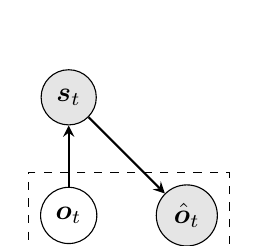
\begin{tikzpicture}[scale=1, transform shape, node distance=1.5cm]
		\node (st) [mcsb] {$\bm{s}_{t} $};
		\node (ot) [mcs, below of=st] {$\bm{o}_{t}$};
		\node (othat) [mcsb, right of=ot] {$\hat{\bm{o}}_{t} $};
		\draw [arrow] (ot) -- (st);
		\draw [arrow] (st) -- (othat);
		\node[draw,dashed,inner sep=1.5mm,fit=(ot) (othat) ] {};
\end{tikzpicture}
\end{center}
		\caption{Auto-encoder: learned by reconstructing the observation (one-to-one).
				The observation is the input and the computed state is the vector at
				the auto-encoder's bottleneck layer, i.e. is the output of the encoder
				part of the auto-encoder network.
		The loss is calculated between the true observation and the reconstructing observation (which
		is obtained by passing the observation though both the encoder and the decoder).}
\end{figure}

\subsection{Forward model}
The auto-encoder does not encode dynamic information.
Since that information is necessary for control, usually a few consequtive
observations (or their embeddings) are stacked and passed to the reinforcement learning algorithm.
This way the information about the dynamics is implicitly provided.
While doing so works, it could be made more efficient by embedding the dynamic
information as well.
One way to achieve this is to trained a model to predict future state representations.
A model can also be observations directly, 
of course provided that the network in question has a bottleneck layer from which
the learned representations can be extracted.
Since learning on sequential information is difficult and would also benefit from
lowering the dimensionality, learning a forward model can be done in two steps:
first, learning an auto-encoder to embed individual frames and then 
learning a predictive model in the embedded space.
In the schematic we show the case where predictions are learned from embeddings
because it is the structurally more complex scheme.
Formally, we have
\begin{equation}
		\hat{\tilde{\bm{s}}}_{ t+1 } = f (\tilde{\bm{s}_{t}}, \bm{a}_{t}; \theta_{ \text{forward} })
\end{equation}
%This however supposes that all states (and the corresponding observations) are accessible 
%prior to the beggining of the training process.
The forward model can be constrained to have linear transition between 
$ \tilde{\bm{s}}_{t}  $ and $ \tilde{\bm{s}}_{t+1}  $, thereby
imposing simple linear dynamics in the learned state space.
Depending on the problem, if this is done well enough, learning a control law can be avoided and instead
schemes like model-predictive control can be employed.

\begin{figure}[htpb]
\begin{center}
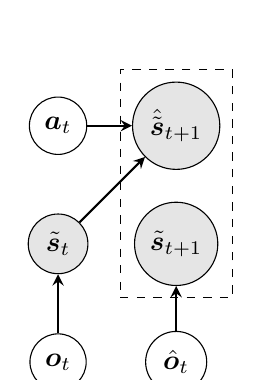
\begin{tikzpicture}[scale=1, transform shape, node distance=1.5cm]
		\node (at) [mcs] {$\bm{a}_{t} $};
		\node (st) [mcsb, below of=at] {$\tilde{\bm{s}}_{t} $};
		\node (sthatplus1) [mcsb, right of=at] {$\hat{\tilde{\bm{s}}}_{t+1} $};
		\node (stplus1) [mcsb, right of=st] {$\tilde{\bm{s}}_{t+1} $};
		\node (ot) [mcs, below of=st] {$\bm{o}_{t}$};
		\node (otplus1) [mcs, right of=ot] {$\hat{\bm{o}}_{t} $};
		\draw [arrow] (at) -- (sthatplus1);
		\draw [arrow] (st) -- (sthatplus1);
		\draw [arrow] (ot) -- (st);
		\draw [arrow] (otplus1) -- (stplus1);
		\node[draw,dashed,inner sep=1.5mm,fit=(sthatplus1) (stplus1) ] {};
\end{tikzpicture}
\end{center}
		\caption{Forward model: predicting the future state from the state-action pair.
				The loss is computer from comparing the predicted state against the true next state
				(the states being the learned states).
				This can also be done directly by predicting the next observation and comparing against it.
				}
\end{figure}



\subsection{Inverse model}
The introducing predictions solves the problem of not embedding the dynamic
information.
However, not all information in the observation is relevant for control.
Consider a computer game where images feature decorative backgrounds ---
those decorations are irrelevant for playing the game well.
If the reconstruction loss is computed from entire observation,
that information is also carried over into the embedded space.
However, if the model is trained to predict actions,
it is only incentivised to use information which the agent can affect.
Thus, due to less information being required,
the inverse model should produce a more compact embedding.
Formally, we can write this as:
\begin{equation}
		\hat{\bm{a}_{t}} = g (\tilde{\bm{s}_{t}}, \tilde{\bm{s}_{t+1}}; \theta_{ \text{inverse} })
\end{equation}
If the inverse model is neural network, we can recover the embedding by discarding
the last few layers and use their outputs to produce the embeddings.

\begin{figure}[htpb]
\begin{center}
\begin{tikzpicture}[scale=1, transform shape, node distance=1.5cm]
		\node (at) [mcs] {$\bm{a}_{t} $};
		\node (athat) [mcsb, below of=at] {$\hat{\bm{a}}_{t} $};
		\node (nothing) [below of=st] {};
		\node (sttilde) [mcsb, left of=nothing] {$\tilde{\bm{s}}_{t} $};
		\node (stildetplus1) [mcsb, right of=nothing] {$\tilde{\bm{s}}_{t+1} $};
		\node (ot) [mcs, below of=sttilde] {$\bm{o}_{t}$};
		\node (otplus1) [mcs, below of=stildetplus1] {$\bm{o}_{t+1} $};
		\draw [arrow] (ot) -- (sttilde);
		\draw [arrow] (otplus1) -- (stildetplus1);
		\draw [arrow] (sttilde) -- (athat);
		\draw [arrow] (stildetplus1) -- (athat);
		\node[draw,dashed,inner sep=1.5mm,fit=(at) (athat) ] {};
\end{tikzpicture}
\end{center}
		\caption{Inverse model: predicting the action between two concequtive states.
				The loss is computer from comparing the predicted action between two consequtive states
				against the true action that
				was taken by the agent between those two states.
				(the states being the learned states).
				}
\end{figure}

\subsection{Using prior knowledge to constrain the state space}
Of course, not everything need be learned in every problem.
While in general hand-engineered features are worse than learned ones,
there are other ways to provide prior knowledge to the learning system.
For example, convolutional neural network by their architecture encode
the fact that nearby pixels are related.
In the SRL context we already mention the possibility of constraining 
the model to linear transitions, but there are other available techniques
like for example
constraining temporal continuity or the principle of causality.
Furthermore, priors can be defined as additional objectives or loss functions.
For example, additional loss can be provided if embeddings from
consequtive observation are drastically different.
This is called the slowness principle.

\subsection{Using hybring objectives}
The approaches outlined thus far can be combined into hybrid
approaches.
TODO: throw a reference or two from the overview paper you're going over,
for example embed2control.

\subsection{Common neural network architectures}
\subsubsection{AE}
Deterministic auto-encoder
\subsubsection{DAE}
Denoising auto-encoder
\subsubsection{VAE}
Variational auto-encoder
\subsubsection{Siamese networks}
Networks that share parameters.

\section{Model-based reinforcement learning}
TODO
Introduce just the idea for the sole purpose of
showing why we aren't doing model-based reinforcement learning,
but instead opting for model-free with state representation learning.


\chapter{Related Work}


As said in the introduction, the goal of the thesis is to use
state representation learning to increase the efficiency 
and finals results of model-free reinforcement learning.
We are now ready to discuss the specifics of our approach.
Firstly, we limit ourselves to image observations and discrete action spaces.In particular, we limit ourselves to Atari57 games as they are common benchmarks in the field for discrete action spaces.\\
As shall be seen in the following sections, some recent work in state-representation learning for  model-free reinforcement learning has been done in robotics problems with continuous action spaces(\cite{yarats},\cite{}, \cite{},).\\

Our goal will mostly be to transfer these successes to the discrete action space setting,namely to DQN and Rainbow algorithms as the basis, instead of SAC and DDPG. In the initial architecture of DQN and Rainbow ,They separately learn state representations from which current observations can be reconstructed, and train a forward model on the learned states. The main limitation of these approaches is the inefficiency of the reconstruction objective, which leads to representations that contain unnecessary information about the observations.

 %---> you sure about that fam??
% maybe do drqv2 but with image reconstruction loss as well?
% yarats didn't try that
Importantly, since we are concerned with finding ways to make  reinforcement learning more sample-efficient, we will be using only off-policy algorithms. Secondly, we are particularly interested in the problem of simultaneous training of the state representations and the policy.
The reason for this is that two-step training is often not available.
This state of affairs is the natural setting for problems where reinforcement learning is a good solution: the problems where exploration is necessary due to either the high complexity of the dynamics or unanticipatable events.
Parallel training of the state representations and the policy necessitates
instability in policy training due to the fact the state estimations
change even for same observations as the state representation are learned.
Hence, related work that focuses on solving or at least ameliorating this issue 
is of particular importance to our work.
Finally, we want our method to be robust not just in the sense that it works
across a wide array of problems, but in the sense that it can be 
easily added to a variety of reinforcement learning algorithms
and yield a positive result. In other words, it should function as a module which can be easily added to new algorithms.
Furthermore, it should work well with other improvements as those suggested in some of the following related work.
For clarity, we divide our discussion of related work in three categories:
prior work on top of which we build, work which utilizes some of the same
techniques we employ for different goal, or which achieves the same goals
in different, but related ways and work which is strongly related to our own from which derived inspiration to our approach.

\section{Work on top of which we build}

As stated in section 2.4.1.6 Integrated agent  was built by integrating the previous extensions of DQN in to one agent.Prioritized replay and multi-step learning were the two most crucial components.compared to the previous benchmarks rainbow was able to improve both  data efficiency and final performance.

TODOs: \cite{sac}
 
The use of deep Auto-Encoder Neural Networks in Reinforcement Learning is till in its early stage.The application of auto-encoders in dimensionality reduction has played a major role in reducing training time and data efficiency
 \cite{auto-encoder for Efficient Embedded Reinforcement Learning}.Introducing auto encoders in batch RL resulted in learning from raw pixels with out previously augmenting the data manually or prepossessing \cite{firstaeinrl}; this closes the  existing gap between the  between the high dimensionality of visual observations and the low dimensionality of state spaces.


\section{Current state-of-the-art on Atari, Agent 57}

Agent 57 \cite{agent57}  was the first deep RL agent that out performs the standard human benchmark on all 57 Atari games.It was built on  on top of the Never Give Up(NGU) agent. which combines two ideas: first, the curiosity-driven exploration, and second, distributed deep RL agents, in particular R2D2.The agent was able to balance the learning of different skills that are required to perform well on such diverse set of games: exploration and exploitation and long-term credit assignment.In order to achieve this a neural network was trained to parameterize a family of policies ranging from very exploratory to purely exploitative,by using adaptive  mechanism polices were prioritized throughout the training process.



\section{Work whose techniques we share}
\begin{enumerate}
		\item (not us, but things that can be done with image loss): \cite{lossisitsownreward}, 
				\cite{rlwauxloss} is the aux loss paper, also uses rewards for aux goals.
				point here is you can use other losses and make them intrinsic rewards.
		\item (us as inspiration) \cite{icm} - here the importance of embedding only
				observations relevant for the agent are discussed.
				they used this to improve exploration though.
\end{enumerate}


\section{Work achieving same goals as us, but differently}
\begin{enumerate}
		\item (not us but same high-level idea): data-augmentation like \cite{drqv1},
				\cite{drqv2}, \cite{rad},
\cite{imageaugmentationisallyouneed},
				contrastive loss like \cite{curl}, 
				\cite{flow}, 
				\cite{invariantrepwithoutreconstruction}
\end{enumerate}
TODO
First explain \cite{rad} which just throws image augmentation over sampled observations.
In \cite{drqv1}, the authors go further by using multiple augmentations over the same image
to regularize the Q-function. The expected return calculated for each of the augmented 
versions of an observation. Then the average of those is calculated and passed
as the predicted expected return. This greatly stabilizes Q-learning
and allows it to learn with much greater sample-efficiency.
Since what is developed is a regularization technique, it can
be seamlessly applied to various reinforcement learning algorithms.
In \cite{drqv2}, the authors futher improve \cite{drqv1} by introducing several
changes to their overall algorithm.

In \cite{curl}, contrastive loss is used instead.


\section{Strongly related to our work}
\begin{enumerate}
		\item 
		\item (us) yarats improving sample efficiency \cite{sac+ae}, \cite{laser}
\end{enumerate}



% METHODS
% CREATED BY DAVID FRISK, 2016
\chapter{Methods }

In this section, we will explain the architecture of our auto-encoder and reinforcement learning algorithm. This includes a description of the environment and preprocessing  in Section 3.0.1., the collection of training data for the auto-encoder and model architecture in section 3.0.2. and the training of the RL agent in Section  3.0.3.


\subsection{Enviroment and Preprocessing}
[!ADD MORE HERE ]

We perform a comprehensive evaluation of our proposed method on the Arcade Learning Environment (Bellemare et al., 2013), which is composed of 57 Atari games. The challenge is to deploy a single algorithm and architecture, with a fixed set of hyper-parameters, to learn to play all the games given embedded latent space representation of the environment from auto encoder and game rewards. This environment is very demanding because it is both comprised of a large number of highly diverse games and the observations are high-dimensional.\\

Working with raw Atari frames, which are 210 x 160 pixel pictures with a 128 color palette, is computationally expensive, therefore we do a basic preprocessing step to reduce the input dimensionality. The raw frames are preprocessed by down sampling to a 110 x 84 picture and transforming their RGB representation to gray-scale.Cropping an 84 x 84 rectangle of the image that nearly captures the playing area yields the final input representation to encoder part of the auto encoder.


\subsection{Deep Auto-encoder and Model Architecture}
[!ADD MORE HERE AFTER NAP]

The first step in the process is to collect data to train the auto-encoder. we run a data collection module to generate the 100000 frame for each stated under the result section.The raw images are transformed to tensors and then trained a variational autoencoder with the objective of re-constructing the original image fed to the network. The auto-encoder was trained for maximum  100 epochs.When reconstructing an image with a network bottleneck, the encoder is forced to compress the original image to a smaller dimensional vector in the latent space.

[By compressing the raw pixels environment to smaller dimensional vector in the latent space we aim to improve the training time it takes for the integrated Rl agent developed by [16] and the shift in the latent space representation and its impact on the RL agent learning performance.We show this in more detail in the following sections.]


\subsection{Training the RL Agent} [!ADD MORE HERE ]

In this paper we integrate auto encoder with integrated agent called Rainbow[12],the selection of this architecture  was based it's ability to out perform all the previous architecture.our main focus was to experiment with the latent space representation of the environment.To address this we set up two experiment architectures one two step training and parallel training.\\

\textbf{Two step Training}: First,we train the auto encoder with the prepossessed data and the weights of the encoder are saved in file for training the agent.In this set up the auto encoder is not updated such that we have a static representation of the environment.

second,we train the integrated agent with the results from the auto encoder.\\

\textbf{Parallel Training}:
In this set up the agent is trained using the dynamic state representation from the encoder as we train both the auto encoder and the integrated agent in parallel.This introduces stochasticity of the environment to the training  and in real life control system we believe that this will set a new paradigm on the use RL.









% RESULTS
% CREATED BY DAVID FRISK, 2016
\chapter{Results}



% CONCLUSION
% CREATED BY DAVID FRISK, 2016
\chapter{Conclusion}
The idea behind this thesis is simple and straightforward:
using autoencoders trained with pixel-reconstruction loss 
to lower the dimensionality of images 
should make the reinforcement learning problem on images easier.
As it turns out, this is not necessarily the case.
It, although unremarkably, works on visually simple games like Pong where
all important details can be capture by MSE loss, i.e. by formulating pixel reconstruction loss
on a pixel-by-pixel basis.
Simultaneously, the same method completely stunts learning on games such as Breakout
where the ball, a crucial element of the state, is captured poorly.

We conclude that and pixel reconstruction loss should be avoided for the purposes of state representation learning
as it does not directly incentivize learning stateful information, but only serve to lower dimensionality,
sometimes even at the expense of stateful information.
This is most exemplified by the fact that forward prediction in pixel space supports learning better,
despite the fact that it maintains an order of magnitude bigger error,
just because it more strongly encourages embedding of stateful information (velocities in particular).
Given the listed reasons, and the gap between our expectations and the obtained results, we recommend 
more research into the nature of features obtained through both unsupervised and reinforcement learning 
so that beneficial combinations can be deduced, rather than guessed.
On a shorter time scale, we recommend discriminative models as both seem more promising 
and are faster in terms of wall-clock time. 


%You may consider to instead divide this chapter into discussion of the results and a summary. 
%
%\section{Discussion}
%
%\section{Conclusion}


% REFERENCES / BIBLIOGRAPHY
\cleardoublepage
\addcontentsline{toc}{chapter}{Bibliography}
\printbibliography

%% CREATED BY DAVID FRISK, 2016
\begin{thebibliography}{69}

\bibitem{Reference}

   [1] Sutton, R. S., \& Barto, A. G. (2018). Reinforcement learning: An introduction. MIT press.\\

  [2]  Mnih, Volodymyr and Kavukcuoglu, Koray and Silver, David and Graves, Alex and Antonoglou, Ioannis and Wierstra, Daan and Riedmiller, Martin.(2013). Playing Atari with Deep Reinforcement Learning.\\

  [3] Mnih, V., Kavukcuoglu, K., Silver, D. et al.(2015). Human-level control through deep reinforcement learning. Nature 518, 529–533.\\

  [4] Hado van Hasselt and Arthur Guez and David Silver.(2015).Deep Reinforcement Learning with Double Q-learning.\\

  [5] van Hasselt.(2010).Double Q-learning. Advances in Neural Information Processing Systems, 23:2613–2621.\\
    
    
  [6] Wang, Ziyu and Schaul, Tom and Hessel, Matteo and van Hasselt, Hado and Lanctot, Marc and de Freitas, Nando.2015.Dueling Network Architectures for Deep Reinforcement Learning.\\
    
    
  [7] Moerland, Thomas M. and Broekens, Joost and Plaat, Aske and Jonker, Catholijn M.Model-based Reinforcement Learning: A Survey.(2020).\\
   
   
  [8] Puterman, M. L. (2014). Markov Decision Processes.: Discrete Stochastic Dynamic Pro- gramming. John Wiley \& Sons.\\
   
   
  [9] M.L. Littman, in International Encyclopedia of the Social \& Behavioral Sciences, 2001.\\
  
  [10]Kidambi et al., 2020
  
  [11] Yu et al., 2021
  
  [12]Ignasi Clavera and Jonas Rothfuss and John Schulman and Yasuhiro Fujita and Tamim Asfour and Pieter Abbeel,
 Model-Based Reinforcement Learning via Meta-Policy Optimization,2018
 
  [13]Duan, J. Schulman, X. Chen, P. L. Bartlett, I. Sutskever, and P. Abbeel. RL$ˆ2$: Fast Reinforcement
Learning via Slow Reinforcement Learning. 11 2016.

  [14]. Sung, L. Zhang, T. Xiang, T. M. Hospedales, and Y. Yang. Learning to learn: Meta-critic networks for
sample efficient learning. CoRR, abs/1706.09529, 2017.

  [15]
  
  [16]Hessel, Matteo and Modayil, Joseph and van Hasselt, Hado and Schaul, Tom and Ostrovski, Georg and Dabney, Will and Horgan, Dan and Piot, Bilal and Azar, Mohammad and Silver, David.2017.Rainbow: Combining Improvements in Deep Reinforcement Learning.
  
  [17]Gerald Tesauro. Temporal difference learning and td-gammon. Communications of the ACM, 38(3):58–68, 1995.
  
  [18]Long-Ji Lin. Reinforcement learning for robots using neural networks. Technical report, DTIC Document, 1993.
  
  [19]Double DQN
  
  [20]Prioritized replay 
  [21]On the use of Deep Auto-encoders for Efficient Embedded Reinforcement Learning







\end{thebibliography}


% APPENDICES
\cleardoublepage
\appendix
\setcounter{page}{1}
\pagenumbering{Roman}			% Capitalized roman numbering starting from I (one)

% CREATED BY DAVID FRISK, 2016
\chapter{Appendix 1}
%(UNFINISED)

%//UPDATE THE FORMAT LATER 
\begin{enumerate}

    \item{ Agent: It is an assumed entity which performs actions in an environment to gain some reward.}
    \item{Environment (e): A scenario that an agent has to face.anything the agent  cannot change arbitrarily is considered to be part of the environment.} 
    \item{Reward (R): An immediate return given to an agent when he or she performs specific action or task.}
    \item{ State (s): State refers to the current situation returned by the environment.}
    \item{Policy ($\pi$): It is a strategy which applies by the agent to decide the next action based on the current state.}
    \item{ Value (V): It is expected long-term return with discount, as compared to the short-term reward.}
    \item{ Value Function: It	specifies the value of a state that is the total amount of reward. It is an agent which should be expected beginning from that state.}
    \item{ Model of the environment: This mimics the behavior of the environment. It helps you to make inferences to be made and also determine how the environment will behave.}
    \item{ Model based methods: It is a method for solving reinforcement learning problems which use model-based methods.}
    \item{ Q value or action value (Q): Q value is quite similar to value. The only difference between the two is that it takes an additional parameter as a current action.}
\end{enumerate}




\end{document}
